%-----------------------------------------------------------------------
% Beginning of chapter.tex
%-----------------------------------------------------------------------
%
%  This is a sample file for use with AMS-LaTeX.  It provides an example
%  of how to set up a file for a book to be typeset with AMS-LaTeX.
%
%  This is the driver file.  Separate chapters should be included at
%  the end of this file.
%
%  ***** DO NOT USE THIS FILE AS A STARTER FOR YOUR BOOK. *****
%  Follow the guidelines in the file chapter.template.
%
%%%%%%%%%%%%%%%%%%%%%%%%%%%%%%%%%%%%%%%%%%%%%%%%%%%%%%%%%%%%%%%%%%%%%%%%

\documentclass[11pt,a4paper]{memoir}
\chapterstyle{demo}
\epigraphfontsize{\small\itshape}
\setlength\epigraphwidth{8cm}
\setlength\epigraphrule{0pt}
\epigraphfontsize{\small\itshape}


%\numberwithin{section}{chapter}
%\numberwithin{figure}{section}

% Include macros here
%=================================================
% Packages
%=================================================

%\usepackage{fixltx2e}
\usepackage[usenames,dvipsnames]{xcolor}
%\usepackage{fancyhdr}
\usepackage{amsmath,amsfonts,amsbsy,amsgen,amscd,mathrsfs,amssymb,amscd}
\usepackage{amsthm}
\usepackage{bm}
\usepackage{url}
\usepackage[UKenglish]{babel}
\usepackage{eurosym}
\usepackage{tikz}
\usepackage{caption}
\usetikzlibrary{matrix,arrows,shapes,calc,3d}
\usepackage{tikz-3dplot}
\tdplotsetmaincoords{60}{110}
\pgfmathsetmacro{\rvec}{.8}
\pgfmathsetmacro{\thetavec}{30}
\pgfmathsetmacro{\phivec}{60}

\tikzset{mynode/.style = {
    % The shape
    circle,
    % The size
    minimum size=2pt,
    % The color
    draw=black, fill=black}
}
\tikzset{vertex/.style={shape=circle, % style for a vertex
                        minimum size=3pt,
                        fill=gray,
                        inner sep = 0pt}}  

% \usepackage{3dplot}
% \tdplotsetmaincoords{60}{110}
%\usepackage{subfig}
\usepackage{microtype}
\usepackage{enumitem}
\usepackage{listings}
\definecolor{darkblue}{rgb}{0,0,.75}

\usepackage[many]{tcolorbox}
\tcbuselibrary{listings}

\definecolor{light-gray}{rgb}{0.96,0.96,0.96}
\definecolor{kwgreen}{rgb}{0,0.5,0}
\definecolor{cogreen}{rgb}{0.25,0.5,0.5}
\definecolor{mygreen}{rgb}{0,0.5,0.125}
\definecolor{equalsign}{rgb}{0.66,0.13,1}
\definecolor{darkred}{rgb}{0.75,0.16,0.37}

\lstloadlanguages{Python} %use listings with Python
%\lstset{literate={==}{{\color{equalsign}==}} {\*}{{\color{equalsign}\*}}}
%\lstnewenvironment{PseudoCode}[1][]
% the space reserved between for the ``In'' numbers and the code
\newlength\inwd
\setlength\inwd{1.7cm}

\newcounter{ipythcntr}

\newtcblisting{ipythonnb}[1][\theipythcntr]{
  enlarge left by=\inwd,
  width=\linewidth-\inwd,
  enhanced,
  boxrule=0.4pt,
  boxsep=0pt,
  left=2pt,
  top=0pt,
  colback=light-gray,
  listing only,
  top=0pt,
  bottom=0pt,
  arc=1pt,
  overlay={
    \node[
      anchor=north east,
      text width=\inwd,
      font=\footnotesize\ttfamily\color{blue!50!black},
      inner ysep=2.5mm,
      inner xsep=0pt,
      outer sep=0pt
      ] 
      at (frame.north west)
      {\stepcounter{ipythcntr}In [#1]:};
  }
  listing style=Python,
  listing options={
    basicstyle=\scriptsize\ttfamily\color{black},
    language=Python,
    escapechar=£,
    showstringspaces=false,
    commentstyle=\color{cogreen},
    keywordstyle=\bfseries\color{kwgreen},
    stringstyle=\color{darkred},
    numberstyle=\color{kwgreen},
    identifierstyle=\color{black},
    %emph={from,import,as},          % Custom highlighting
    otherkeywords={0,1,2,3,4,5,6,7,8,9,\*,==,<=,>=,+,-,\%},
    emph={*,==,<=,>=,+,-,\%},    
    emphstyle=\color{equalsign},
    extendedchars=true,
  },
}

\newtcblisting{ipythonnbout}[1][\theipythcntr]{
  enlarge left by=\inwd,
  width=\linewidth-\inwd,
  enhanced,
  boxrule=0pt,
  boxsep=0pt,
  left=2pt,
  top=0pt,
  colback=white,
  listing only,
  top=0pt,
  bottom=0pt,
  frame hidden,
  overlay={
    \node[
      anchor=north east,
      text width=\inwd,
      font=\footnotesize\ttfamily\color{red},
      inner ysep=2.5mm,
      inner xsep=0pt,
      outer sep=0pt
      ] 
      at (frame.north west)
      {\stepcounter{ipythcntr}Out [#1]:};
  }
  listing style=Python,
  listing options={
    basicstyle=\scriptsize\ttfamily\color{black},
    language=Python,
    escapechar=£,
    showstringspaces=false,
    commentstyle=\color{cogreen},
    keywordstyle=\bfseries\color{kwgreen},
    stringstyle=\color{darkred},
    numberstyle=\color{kwgreen},
    identifierstyle=\color{black},
    %emph={from,import,as},          % Custom highlighting
%    otherkeywords={as,0,1,2,3,4,5,6,7,8,9,\*,==,<=,>=,+,-},
%    emph={*,==,<=,>=,+,-},    
%    emphstyle=\color{equalsign},
    extendedchars=true,
    %literate={#}{{\#}},
  },
}

\newtcblisting{ipythonnboutno}{
  enlarge left by=\inwd,
  width=\linewidth-\inwd,
  enhanced,
  boxrule=0pt,
  boxsep=0pt,
  left=2pt,
  top=0pt,
  colback=white,
  listing only,
  top=0pt,
  bottom=0pt,
  frame hidden,
  overlay={
    \node[
      anchor=north east,
      text width=\inwd,
      font=\footnotesize\ttfamily\color{red},
      inner ysep=2.5mm,
      inner xsep=0pt,
      outer sep=0pt
      ] 
      at (frame.north west)
      {};
  }
  listing style=Python,
  listing options={
    basicstyle=\scriptsize\ttfamily\color{black},
    language=Python,
    escapechar=£,
    showstringspaces=false,
    commentstyle=\color{cogreen},
    %keywordstyle=\bfseries\color{kwgreen},
    stringstyle=\color{darkred},
    numberstyle=\color{kwgreen},
    identifierstyle=\color{black},
    %emph={from,import,as},          % Custom highlighting
    %otherkeywords={as,0,1,2,3,4,5,6,7,8,9,\[,\]},
    %emph={[,]},    
    %emphstyle=\color{black},
    extendedchars=true,
    %literate={#}{{\#}},
  },
}


%{\lstset{language=Matlab,basicstyle=\small, keywordstyle=\color{darkblue},numbers=none,xleftmargin=.04\textwidth,mathescape,frame=single,#1}}
%{}
%\usepackage[]{algorithm2e}
%\usepackage{mcode}
\usepackage{multicol}

%\usepackage[draft]{changes}
%\definechangesauthor[color=blue]{ml}
%\definechangesauthor[color=red]{da}
% \usepackage{trackchanges}
% \addeditor{ml}
% \addeditor{da}

\definecolor{dark-gray}{gray}{0.3}
\definecolor{dkgray}{rgb}{.4,.4,.4}
\definecolor{dkblue}{rgb}{0,0,.5}
\definecolor{medblue}{rgb}{0,0,.75}
\definecolor{rust}{rgb}{0.5,0.1,0.1}

\usepackage[colorlinks=true]{hyperref}
\hypersetup{urlcolor=Blue}
\hypersetup{citecolor=Black}
\hypersetup{linkcolor=dark-gray}

%\usepackage{setspace}
\usepackage{graphicx}
%\usepackage{multicol}
\usepackage{booktabs,longtable,tabu} % Nice tables
\setlength{\tabulinesep}{1pt}
\usepackage{multirow} % More control over tables
\usepackage{float}
\usepackage[T1]{fontenc}
%\usepackage{quotchap}

% Fonts
\usepackage{times}
%\usepackage{fourier}
%\usepackage[no-math]{fontspec}
%\setmainfont{optima}
%\usepackage{charter}
\usepackage{bm} % boldmath must be called after the package

%=================================================
% Paths
%=================================================

\graphicspath{{figures/}}

%=================================================
% Formatting
%=================================================

%\sloppy % Helps with margin justification

%%% Further font changes
\newcommand{\lang}{\textit}
\newcommand{\titl}{\textsl}
\newcommand{\term}{\emph}

%%% Equation numbering
\numberwithin{equation}{section} 

%%% Typesetting
\providecommand{\mathbold}[1]{\bm{#1}}  % Must be after 'fourier'
                                % package loads
%%% Annotations
\newcommand{\notate}[1]{\textcolor{red}{\textbf{[#1]}}}

%=================================================
% Theorem environment
%=================================================

\newtheorem{bigthm}{Theorem}
\renewcommand{\thebigthm}{\Roman{bigthm}}

\newtheorem{theorem}{Theorem}[section]
\newtheorem{lemma}[theorem]{Lemma}
\newtheorem{sublemma}[theorem]{Sublemma}
\newtheorem{proposition}[theorem]{Proposition}
\newtheorem{fact}[theorem]{Fact}
\newtheorem{result}[theorem]{Result}
\newtheorem{conjecture}[theorem]{Conjecture}
\newtheorem{corollary}[theorem]{Corollary}

\newtheorem{problem}[theorem]{Problem}
\newtheorem{solution}[theorem]{Solution}

\theoremstyle{definition}

\newtheorem{definition}[theorem]{Definition}
\newtheorem{example}[theorem]{Example}
\newtheorem{remark}[theorem]{Remark}

\newenvironment{mainthm}{\par\textsc{Main theorem.}\it}{\par}
\renewcommand{\thebigthm}{\Alph{bigthm}}

%=================================================
% Symbols
%=================================================

%%% Old symbols with new names
\newcommand{\oldphi}{\phi}
\renewcommand{\phi}{\varphi}

\newcommand{\eps}{\varepsilon}
\newcommand{\e}{\varepsilon}

%\newcommand{\oldmid}{\mid}
\renewcommand{\mid}{\mathrel{\mathop{:}}} 

%%% New symbols
\newcommand{\defby}{\overset{\mathrm{\scriptscriptstyle{def}}}{=}}
\newcommand{\half}{\tfrac{1}{2}}
\newcommand{\third}{\tfrac{1}{3}}

\newcommand{\sumnl}{\sum\nolimits}

\newcommand{\defeq}{\ensuremath{\mathrel{\mathop{:}}=}} % Definition-equals
\newcommand{\eqdef}{\ensuremath{=\mathrel{\mathop{:}}}} % Equals-definition

%%% Constants
\newcommand{\cnst}[1]{\mathrm{#1}} 
\newcommand{\econst}{\mathrm{e}}
\newcommand{\iunit}{\mathrm{i}}

\newcommand{\onevct}{\mathbf{e}} % All ones vector
\newcommand{\zerovct}{\vct{0}} % Zero vector

\newcommand{\Id}{\mathbf{I}}
\newcommand{\onemtx}{\bm{1}}
\newcommand{\zeromtx}{\bm{0}}

%%% Sets
\newcommand{\coll}[1]{\mathscr{#1}}
\newcommand{\sphere}[1]{S^{#1}}
\newcommand{\ball}[1]{B^{#1}}
\newcommand{\Grass}[2]{\mathbb{G}(#1,#2)}
\providecommand{\mathbbm}{\mathbb} % In case we don't load bbm
\newcommand{\Rplus}{\mathbbm{R}_{+}}
\newcommand{\R}{\mathbbm{R}}
\newcommand{\C}{\mathbbm{C}}
\newcommand{\N}{\mathbbm{N}}
\newcommand{\FF}{\mathbbm{F}}
\newcommand{\struct}{\mathcal{S}}

% Group theory
\newcommand{\stab}{\mathrm{stab}}

% Algebra
\newcommand{\End}{\mathrm{End}}
\newcommand{\Hom}{\mathrm{Hom}}
\newcommand{\Mult}{\mathrm{Mult}}

% Set operations
\newcommand{\polar}{\circ}
\newcommand{\closure}{\overline}
\newcommand{\prtensor}{\,\hat{\otimes}\,}

%%% Real and complex analysis
\newcommand{\abs}[1]{\left\vert {#1} \right\vert}
\newcommand{\abssq}[1]{{\abs{#1}}^2}

\newcommand{\sgn}[1]{\operatorname{sgn}{#1}}
\newcommand{\real}{\operatorname{Re}}
\newcommand{\imag}{\operatorname{Im}}
\newcommand{\pos}{\operatorname{Pos}}
\newcommand{\shrink}{\operatorname{Shrink}}

\newcommand{\diff}[1]{\mathrm{d}{#1}}
\newcommand{\idiff}[1]{\, \diff{#1}}

\newcommand{\gradd}{\mathrm{grad }} % Conflicts w/SIAM styles?
\newcommand{\divv}{\mathrm{div }}
\newcommand{\subdiff}{\partial}

%%% Optimization

\newcommand{\minimize}{\text{minimize}\quad}
\newcommand{\maximize}{\text{maximize}\quad}
\newcommand{\subjto}{\quad\text{subject to}\quad}
\newcommand{\find}{\text{find}\quad}
\newcommand{\suchthat}{\quad\text{such that}\quad}

\newcommand{\argmin}{\operatorname*{arg\; min}}
\newcommand{\argmax}{\operatorname*{arg\; max}}
\newcommand{\dom}{\mathrm{dom} }

%%% Probability & measure

\newcommand{\Prob}{\mathbbm{P}}
\newcommand{\Probe}[1]{\Prob\left({#1}\right)}
\newcommand{\Expect}{\operatorname{\mathbb{E}}}

\newcommand{\St}{\operatorname{St}}

%\newcommand{\normal}{\textsc{Normal}}
\newcommand{\normal}{N}
\newcommand{\uniform}{\textsc{Uniform}}
\newcommand{\erf}{\operatorname{erf}}

\DeclareMathOperator{\rvol}{rvol}
\DeclareMathOperator{\Var}{Var}
\DeclareMathOperator{\Gl}{Gl}
\newcommand{\diag}{\operatorname{diag}}

%%% Vector and matrix operators
\newcommand{\vct}[1]{\mathbold{#1}}
\newcommand{\mtx}[1]{\mathbold{#1}}
\newcommand{\Eye}{\mathbf{I}}

\newcommand{\transp}[1]{#1^{T}}
\newcommand{\trans}{\top}
\newcommand{\adj}{*}
\newcommand{\psinv}{\dagger}

\newcommand{\lspan}[1]{\operatorname{span}{#1}}

\newcommand{\range}{\operatorname{range}}
\newcommand{\colspan}{\operatorname{colspan}}

%\newcommand{\rank}{\operatorname{rank}}
\newcommand{\nullity}{\operatorname{null}}
%\newcommand{\ker}{\operatorname{ker}}
\newcommand{\im}{\operatorname{im}}
%\newcommand{\span}{\operatorname{span}}

%\newcommand{\diag}{\operatorname{diag}}
\newcommand{\trace}{\operatorname{tr}}

\newcommand{\supp}[1]{\operatorname{supp}(#1)}
\newcommand{\sign}[1]{\operatorname{sign}(#1)}

\newcommand{\smax}{\sigma_{\max}}
\newcommand{\smin}{\sigma_{\min}}

\newcommand{\nnz}{\operatorname{nnz}}
\renewcommand{\vec}{\operatorname{vec}}

\newcommand{\Proj}{\ensuremath{\mtx{\Pi}}} % Projection operator

%%% Semidefinite orders
\newcommand{\psdle}{\preccurlyeq}
\newcommand{\psdge}{\succcurlyeq}

\newcommand{\psdlt}{\prec}
\newcommand{\psdgt}{\succ}

%%% Mensuration: inner products and norms

% TeX does not like either \newcommand or \renewcommand for these
% two macros.  There is probably a good reason not to use them via
% \def, but I don't know it.  
%\newcommand{\<}{\langle} 
%\newcommand{\>}{\rangle}
\newcommand{\ip}[2]{\langle {#1}, {#2} \rangle}
% --deleted the \left and \right-- Dennis
% \newcommand{\ip}[2]{\left\langle {#1},\ {#2} \right\rangle}
\newcommand{\absip}[2]{\abs{\ip{#1}{#2}}}
\newcommand{\abssqip}[2]{\abssq{\ip{#1}{#2}}}
\newcommand{\tworealip}[2]{2 \, \real{\ip{#1}{#2}}}

%\newcommand{\norm}[1]{\left\Vert {#1} \right\Vert}
\newcommand{\norm}[1]{\Vert {#1}\Vert}
\newcommand{\normsq}[1]{\norm{#1}^2}

\newcommand{\lone}[1]{\norm{#1}_{\ell_1}}
\newcommand{\smlone}[1]{\|#1\|_{\ell_1}}
\newcommand{\linf}[1]{\norm{#1}_{\ell_\infty}}
\newcommand{\sone}[1]{\norm{#1}_{S_1}}
\newcommand{\snorm}[1]{\sone{#1}}
\newcommand{\wnnorm}[1]{\norm{#1}_{*,\vct{w}}}
\newcommand{\wnnormd}[1]{\norm{#1}^*_{\vct{w}}}
\DeclareMathOperator{\dist}{dist}

% Fixed-size inner products and norms are useful sometimes
\newcommand{\smip}[2]{\bigl\langle {#1}, \ {#2} \bigr\rangle}
\newcommand{\smabsip}[2]{\bigl\vert \smip{#1}{#2} \bigr\vert}
\newcommand{\smnorm}[2]{{\bigl\Vert {#2} \bigr\Vert}_{#1}}

% Specific norms that are used frequently
\newcommand{\enormdangle}{{\ell_2}}
\newcommand{\enorm}[1]{\norm{#1}}
\newcommand{\enormsm}[1]{\enorm{\smash{#1}}}

\newcommand{\enormsq}[1]{\enorm{#1}^2}

\newcommand{\fnorm}[1]{\norm{#1}_{\mathrm{F}}}
\newcommand{\fnormsq}[1]{\fnorm{#1}^2}

\newcommand{\pnorm}[2]{\norm{#2}_{#1}}
%\newcommand{\snorm}[1]{\norm{#1}_*}

\newcommand{\triplenorm}[1]{\left\vert\!\left\vert\!\left\vert {#1} \right\vert\!\right\vert\!\right\vert} 

\newcommand{\flag}[2]{{#1 \brack #2}}

% Special cones
\newcommand{\Feas}{\mathcal{F}}
\newcommand{\Desc}{\mathcal{D}}

\newcommand{\sdim}{\delta}
\newcommand{\sdimw}{\delta^*}
% \newcommand{\sdimw}{\tilde{\delta}}
\newcommand{\ddt}[1]{\dot{#1}}
\DeclareMathOperator{\Circ}{Circ}

%%% Differential geometry
\newcommand{\Cinf}{C^{\infty}}
\newcommand{\Tensf}{\mathcal{T}}
\newcommand{\Vbundle}{\mathcal{X}}
\newcommand{\Christ}[3]{\Gamma_{{#1}{#2}}^{#3}}

% Stuff to be sorted in somewhere
\DeclareMathOperator{\Lip}{Lip}

\newcommand{\IR}{\mathbbm{R}}
\newcommand{\veps}{\varepsilon}
\newcommand{\mA}{\mathcal{A}}
\newcommand{\mB}{\mathcal{B}}
\newcommand{\mC}{\mathcal{C}}
\newcommand{\mD}{\mathcal{D}}
\newcommand{\mE}{\mathcal{E}}
\newcommand{\mI}{\mathcal{I}}
\newcommand{\mM}{\mathcal{M}}
\newcommand{\mN}{\mathcal{N}}
\newcommand{\mL}{\mathcal{L}}
\newcommand{\mV}{\mathcal{V}}
\newcommand{\bface}{\overline{\mathcal{F}}}
\newcommand{\face}{\mathcal{F}}
\newcommand{\relint}{\operatorname{relint}}
\newcommand{\relcl}{\operatorname{relcl}}
\newcommand{\cone}{\operatorname{cone}}
\newcommand{\lin}{\operatorname{lin}}
\newcommand{\Gr}{\operatorname{Gr}}
\newcommand{\powerset}{\mathscr{P}}
\newcommand{\hd}{{\operatorname{hd}}}
\newcommand{\inter}{{\operatorname{int}}}
\newcommand{\conv}{\operatorname{conv}}
\newcommand{\clconv}{\overline{\conv}}
\newcommand{\cl}{\operatorname{cl}}
\newcommand{\bd}{\operatorname{bd}}

\newcommand{\GL}{\operatorname{GL}}

% \newcommand{\tb}{\stackrel{0}{\to}}
\newcommand{\tb}{\,\,\mathring{\to}\,\,}
% \newcommand{\tdash}{\,\,\overset{e}{\to}\,\,}
% \newcommand{\tdash}{\,\,\overset{a}{\to}\,\,}
\newcommand{\tdash}{\overset{a}{\to}}

\newcommand{\K}{\mathcal{K}}
\newcommand{\B}{\mathcal{B}}
\newcommand{\F}{\mathcal{F}}
\newcommand{\D}{\mathcal{D}}
\renewcommand{\P}{\mathcal{P}}
\DeclareMathOperator{\id}{id}
\DeclareMathOperator{\gr}{gr}
\newcommand{\vp}{\varphi}
\newcommand{\maxp}{{\max}_p}
\DeclareMathOperator{\spa}{span}
\DeclareMathOperator{\vol}{vol}
\DeclareMathOperator{\ima}{im}
\DeclareMathOperator{\rk}{rk}

\newcommand{\Ren}{\mathcal{R}}
\newcommand{\T}{\mathcal{T}}
% ADJUST THE FOLLOWING
% \newcommand{\resTMP}[2]{#1,#2}
\newcommand{\resTMP}[2]{#1\to#2}
% 
\newcommand{\res}[3]{\vct{#1}_{\resTMP{#2}{#3}}}
\newcommand{\nres}[3]{\|\vct{#1}\|_{\resTMP{#2}{#3}}}
\newcommand{\sres}[3]{\sigma_{\resTMP{#2}{#3}}(\vct{#1})}
\newcommand{\csres}[3]{\overline{\sigma}_{\resTMP{#2}{#3}}(\vct{#1})}
\newcommand{\kres}[3]{\kappa_{\resTMP{#2}{#3}}(\vct{#1})}
% transpose
\newcommand{\rest}[3]{\vct{#1}^T_{\resTMP{#2}{#3}}}
\newcommand{\nrest}[3]{\|\vct{#1}^T\|_{\resTMP{#2}{#3}}}
\newcommand{\srest}[3]{\sigma_{\resTMP{#2}{#3}}(\vct{#1}^T)}
\newcommand{\csrest}[3]{\overline{\sigma}_{\resTMP{#2}{#3}}(\vct{#1}^T)}
\newcommand{\srestm}[3]{\sigma_{\resTMP{#2}{#3}}(-\vct{#1}^T)}
\newcommand{\krest}[3]{\kappa_{\resTMP{#2}{#3}}(\vct{#1}^T)}
\newcommand{\nresdag}[3]{\|\vct{#1}^\dagger\|_{\resTMP{#2}{#3}}}

\newcommand{\RCD}[3]{\Ren_{#2,#3}(\vct{#1})}
% \newcommand{\RCD}[3]{\Ren_{\resTMP{#2}{#3}}(\vct{#1})}

\newcommand{\DA}{\vct{\Delta A}}

%
\newcommand{\Rmm}{R_{\mathrm{mm}}}

\newcommand{\rbinom}[2]{\genfrac{[}{]}{0pt}{}{#1}{#2}}
\newcommand{\trbinom}[2]{{\textstyle\genfrac{[}{]}{0pt}{}{#1}{#2}}}

\newcommand{\comm}[1]{\textcolor{red}{\textbf{[#1]}}}
\newcommand{\rant}[1]{\textcolor{blue}{\textbf{[#1]}}}
%

\newcommand{\llangle}{\langle\hspace{-1.5pt}\langle}  % this is actually contained in mnsymbol, but loading this package causes trouble...
\newcommand{\rrangle}{\rangle\hspace{-1.5pt}\rangle}  % this is actually contained in mnsymbol, but loading this package causes trouble...

\newcommand{\Res}{\mathrm{Res}}
\newcommand{\Oh}{\mathcal{O}}
\newcommand{\Mbar}{\overline{M}}
\newcommand{\second}{\mathrm{II}}
\newcommand{\nablabar}{\overline{\nabla}}
\newcommand{\expm}{\mathrm{exp}}
\newcommand{\Rc}{\mathrm{Rc}}
\newcommand{\NJ}{\mathrm{NJ}}
% %\newcommand{\GL}[1]{\mathrm{GL}(#1)}

\newcommand{\cover}{\lessdot}

% Semidefinite programming
\newcommand{\Sym}{\mathcal{S}}
\newcommand{\SDP}{\mathcal{S}_+}
\newcommand{\psd}{\succeq}
\newcommand{\bdot}{\bullet}
\marginparmargin{outer}
%\renewcommand{\chaptername}{}
%\renewcommand{\thechapter}{}
\newtheorem*{theorem*}{Theorem}
\renewcommand{\thesection}{\arabic{section}}

\renewcommand\thefigure{\thesection.\arabic{figure}}

\begin{document}

\chapter*{Background Material}
\addcontentsline{toc}{chapter}{Background Material}
These notes contain a summary of background material from linear algebra and calculus. Much of the content should be familiar to some degree, and the purpose is to bring it back to attention. Important concepts are \textbf{highlighted} in the notes.

\section{Asymptotic notation}
An \marginpar{\textbf{algorithm}}\textbf{algorithm} is a sequence of instructions carried out by a computer. Important features of an algorithm are computation time (measured as the number of operations or the number of iterations needed to reach a solution) and accuracy. 
One is mainly interested in the \marginpar{\textbf{orders of magnitude}}\textbf{orders of magnitude} of these quantities, and not so much in their exact values. A convenient notation for this purpose is the asymptotic O-notation.

Let $f,g\colon \R\to \R$ be two functions. Then:
\begin{itemize}
 \item $f(n)\in O(g(n))$ as $n\to \infty$ if there exists a constant $C>0$ and an integer $n_0$ such that $|f(n)|\leq C |g(n)|$ for $n>n_0$;\marginpar{$O(g(n))$, $O(g(x))$}
 \item $f(x)\in O(g(x))$ as $x\to 0$ if there exists a constant $C>0$ and a real number $\e>0$ such that $|f(x)|\leq C|g(x)|$ for $|x|<\e$.
\end{itemize}

We omit ``$n\to \infty$'' or ``$x\to 0$'' when it is clear from the context. One often finds statements such as $f(n)=O(g(n))$ or $f(x) = 1+x+O(x^2)$; the first is equivalent to $f(n)\in O(g(n))$, while the second should be read as $f(x) = 1+x+g(x)$ for a function $g(x)\in O(x^2)$.
% Note that the order does not change when multiplying an expression by a constant. The order of a sum of expressions as $n\to \infty$ is the order of the fastest growing term. For example,
% $\log^2(n)+n^2+0.1n^3 \in O(n^3)$ as $n\to \infty$.
% Similarly, the order the order of a sum of expressions as $x\to 0$ is the order of the largest term as $x\to 0$. 
The following examples illustrate the O-notation.

\begin{figure}[h!]
\begin{minipage}{0.45\textwidth}
 \begin{itemize}
 \item $\sqrt{n}+n^2\in O(n^2)$ as $n\to \infty$
 \item $n^5\in O(e^{n})$ as $n\to \infty$
 \item $10^{100}\in O(1)$ as $n\to \infty$
 \end{itemize}
\end{minipage}
%
\begin{minipage}{0.45\textwidth}
  \begin{itemize}
 \item $x^3\in O(x^2)$ as $x\to 0$
 \item $\sin(x) \in O(x)$ as $x\to 0$
 \item $e^x = 1+x+O(x^2)$ as $x\to 0$
 \end{itemize}
\end{minipage}
\end{figure}

The notation $f(n)\in \Omega(g(n))$ as $n\to \infty$ means that $g(n)\in O(f(n))$ as $n\to \infty$, and $f(n)\in o(g(n))$ as $n\to \infty$ means that for {\em all} $C>0$ there exists $n_0$ such that $|f(n)|<C|g(n)|$ for $n>n_0$. If $g(n)\neq 0$ for sufficiently large $n$, this is equivalent to $\lim_{n\to \infty}\frac{f(n)}{g(n)} = 0$. One defines $\Omega(g(x))$ and $o(g(x))$  as $x\to 0$ analogously.

\section{Linear Algebra}
We restrict to linear algebra over the field of real numbers $\R$, as this is the setting that is of most interest in optimization. A \marginpar{\textbf{vector}}\textbf{vector} in $\R^n$ and its \marginpar{\textbf{transpose}}\textbf{transpose} are written as
\begin{equation*}
  \vct{x} = \begin{pmatrix} x_{1}\\
                    \vdots\\
                    x_{n}
\end{pmatrix} = (x_1,\dots,x_n)^{\trans}, \quad 
  \vct{x}^\trans = (x_{1}, \dots, x_{n}),
\end{equation*}
with \marginpar{\textbf{coordinates}}\textbf{coordinates} $x_i\in \R$ for $1\leq i\leq n$. The zero vector is denoted by $\zerovct$, while $\vct{e}$ is the vector with every coordinate equal to $1$. If $\lambda_1,\lambda_2\in \R$ and $\vct{x},\vct{y}\in \R^n$, then $\lambda_1 \vct{x}+\lambda_2\vct{y}$ is the vector with coordinates $\lambda_1x_i+\lambda_2y_i$ for $1\leq i\leq n$.

In $\R^n$ we have the Euclidean (or standard) \marginpar{\textbf{inner product}}\textbf{inner product} (or scalar product)
\begin{equation*}
 \ip{\vct{x}}{\vct{y}} = \sum_{i=1}^n x_i y_i.
\end{equation*}
The Euclidean inner product is \marginpar{\textbf{bilinear}}\textbf{bilinear}: for $\vct{x}_1,\vct{x}_2,\vct{y}_1,\vct{y}_2\in \R^n$ and $\alpha,\beta\in \R$,
\begin{equation*}
 \ip{\alpha \vct{x}_1+\beta \vct{x}_2}{\vct{y}} = \alpha\ip{\vct{x}_1}{\vct{y}}+\beta\ip{\vct{x}_2}{\vct{y}}, \quad \ip{\vct{x}}{\alpha \vct{y}_1+\beta \vct{y}_2} = \alpha\ip{\vct{x}}{\vct{y}_1}+\beta\ip{\vct{x}}{\vct{y}_2}, 
\end{equation*}
symmetric ($\ip{\vct{x}}{\vct{y}}=\ip{\vct{y}}{\vct{x}}$) and satisfies $\ip{\vct{x}}{\vct{x}}\geq 0$, with equality if and only if $\vct{x}=\zerovct$.
Two vectors $\vct{x}$ and $\vct{y}$ are called \marginpar{\textbf{orthogonal}}\textbf{orthogonal}, if $\ip{\vct{x}}{\vct{y}}=0$. 

\begin{example}
 The vectors $(1,1)^{\trans}$ and $(1,-1)^{\trans}$ are orthogonal in $\R^2$, while $(1,1)^{\trans}$ and $(2,-1)^{\trans}$ are not.
 
\begin{minipage}{0.45\textwidth}
\centering
\begin{tikzpicture}[thick,rotate=0,scale=0.7]
\node (A1) at (0.7,0.7)  [label=45:{$(1,1)^{\trans}$}] {};
\node (A2) at (0.7,-0.7)  [label=-45:{$(1,-1)^{\trans}$}] {};
\draw[color=black, thick, <-] (1,1) -- (0,0);
\draw[color=black, thick, <-] (1,-1) -- (0,0);
\draw[color=gray, dashed, ->] (-2,0) -- (2,0);
\draw[color=gray, dashed, ->] (0,-2) -- (0,2);
\draw[color=gray] (-0.1,1) -- (0.1,1);
\draw[color=gray] (-0.1,-1) -- (0.1,-1);
\draw[color=gray] (1,-0.1) -- (1,0.1);
\draw[color=gray] (-1,-0.1) -- (-1,0.1);
\end{tikzpicture}
\captionof{figure}{Orthogonal vectors} \label{fig:orth}
\end{minipage}
%
\begin{minipage}{0.45\textwidth}
\centering
\begin{tikzpicture}[thick,rotate=0,scale=0.7]
\node (A1) at (0.7,0.7)  [label=45:{$(1,1)^{\trans}$}] {};
\node (A2) at (1.7,-0.7)  [label=-45:{$(2,-1)^{\trans}$}] {};
\draw[color=black, thick, <-] (1,1) -- (0,0);
\draw[color=black, thick, <-] (2,-1) -- (0,0);
\draw[color=gray, dashed, ->] (-2,0) -- (2,0);
\draw[color=gray, dashed, ->] (0,-2) -- (0,2);
\draw[color=gray] (-0.1,1) -- (0.1,1);
\draw[color=gray] (-0.1,-1) -- (0.1,-1);
\draw[color=gray] (1,-0.1) -- (1,0.1);
\draw[color=gray] (-1,-0.1) -- (-1,0.1);
\end{tikzpicture}
\captionof{figure}{Non-orthogonal vectors} \label{fig:north}
\end{minipage}
\end{example}

\subsection{Linear subspaces}
A \marginpar{\textbf{linear subspace}}\textbf{linear subspace} is a subset $V\subseteq \R^n$ such that for any $\vct{x},\vct{y}\in V$ and for all $\alpha,\beta\in \R$, $\alpha \vct{x}+\beta \vct{y}\in V$. In particular, the sets $\{\zerovct\}$ and $\R^n$ are linear subspaces. 

\begin{example}
The linear subspaces of $\R^2$ are $\{\zerovct\}$, lines through the origin, and $\R^2$. The linear subspaces of $\R^3$ are $\{\zerovct\}$, lines and planes through the origin, and $\R^3$.
\end{example}

A \marginpar{\textbf{linear combination}}\textbf{linear combination} of vectors $\vct{x}_1,\dots,\vct{x}_k\in \R^n$ 
is an expression of the form $\vct{x}=\sum_{i=1}^k \lambda_i \vct{x}_i$, where $\lambda_i\in \R$ for $1\leq i\leq k$. The set of linear combinations
\begin{equation*}
 V = \mathrm{span}\ \{\vct{x}_1,\dots,\vct{x}_k\} := \left\{\sum_{i=1}^k \lambda_i \vct{x}_i \mid \lambda_i\in \R\right\}
\end{equation*}
forms a linear subspace of $\R^n$. It is the intersection of all linear subspaces that contain $\vct{x}_1,\dots,\vct{x}_k$. 
The vectors $\vct{x}_1,\dots,\vct{x}_k$ are \marginpar{\textbf{linearly independent}}\textbf{linearly independent} if $\sum_{i=1}^k \lambda_i\vct{x}_i=0$ implies $\lambda_1=\cdots=\lambda_k=0$. A minimal set of vectors that span a linear subspace $V$ is called
a \marginpar{\textbf{basis}}\textbf{basis} of this subspace, and the number of elements in a basis is the \marginpar{\textbf{dimension}}\textbf{dimension} of the linear subspace. The elements of a basis are always linearly independent, and a maximal linearly independent set in a vector subspace $V$ is a basis.
If $\{\vct{b}_1,\dots,\vct{b}_k\}$ is a basis of a subspace $V$, then every $\vct{x}\in V$ has a {\em unique} representation $\vct{x}=\sum_{i=1}^k \lambda_i \vct{b}_i$.
A basis is \marginpar{\textbf{orthonormal basis}}\textbf{orthogonal} if $\ip{\vct{b}_i}{\vct{b}_j}=0$ for $i\neq j$, and \textbf{orthonormal} if in addition $\ip{\vct{b}_i}{\vct{b}_i}=1$ for $1\leq i\leq k$. The unique expression of $\vct{x}\in V$ as linear combination of an orthonormal basis $\{\vct{b}_1,\dots,\vct{b}_k\}$ of $V$ is given by
\begin{equation*}
 \vct{x} = \sum_{i=1}^k \ip{\vct{x}}{\vct{b}_i} \vct{b}_i.
\end{equation*}
The \marginpar{\textbf{standard basis}}\textbf{standard basis} of $\R^n$ is the orthonormal basis $\{\vct{e}_1,\dots,\vct{e}_n\}$, where $\vct{e}_i$ has a $1$ in the $i$-th coordinate and $0$ elsewhere.

\begin{example}\label{ex:23}
The vectors $\vct{v}_1 = (0,1,1)^{\trans}$ and $\vct{v}_2 = (1,0,1)^{\trans}$
span a linear subspace of $\R^3$ of dimension $2$, but they are not orthogonal. The vectors 
\begin{equation*}
\vct{b}_1 = \frac{1}{\sqrt{2}}\begin{pmatrix}
0\\1\\1
\end{pmatrix}, 
\vct{b}_2 = \frac{1}{\sqrt{3}}\begin{pmatrix}
\sqrt{2}\\-\frac{1}{\sqrt{2}}\\ \frac{1}{\sqrt{2}}
\end{pmatrix}
\end{equation*}
form an orthonormal basis of $V$. The vector $\vct{x}=(1,1,2)^{\trans}$ lives in $V$, and its representation in terms of $\{\vct{b}_1,\vct{b}_2\}$ is
\begin{equation*}
\vct{x} = \frac{3}{\sqrt{2}}\vct{b}_1 + \sqrt{\frac{3}{2}}\vct{b}_2.
\end{equation*}

\begin{figure}[h!]
\centering
\begin{tikzpicture}[scale=3,tdplot_main_coords]

%set up some coordinates 
%-----------------------
\coordinate (O) at (0,0,0);
\coordinate (B1) at (0,{sqrt(0.5)},{sqrt(0.5)});
\coordinate (B2) at ({sqrt(0.67)},-{sqrt(0.167)},{sqrt(0.167)});

%draw figure contents
%--------------------
\filldraw[fill=red!20] (O) -- (B1) -- (B2) -- (O) -- cycle; 

%draw the main coordinate system axes
\draw[thin,->] (O) -- (1,0,0) node[anchor=north east]{$x$};
\draw[thin,->] (O) -- (0,1,0) node[anchor=north west]{$y$};
\draw[thin,->] (O) -- (0,0,1) node[anchor=south]{$z$};

%draw points v_1 and v_2
\draw[thick,->] (O) -- (0,1,1) node[anchor=north west]{$\vct{v}_1$};
\draw[thick,->] (O) -- (1,0,1) node[anchor=north east]{$\vct{v}_2$};
\draw[thick,->,color=blue] (O) -- (B1) node[anchor=north west]{$\vct{b}_1$};
\draw[thick,->,color=blue] (O) -- (B2) node[anchor=north]{$\vct{b}_2$};
\end{tikzpicture}
\end{figure}
\end{example}

The \marginpar{\textbf{direct sum} $\oplus$}\textbf{direct sum} of two vector subspaces $V,W\subset \R^n$ with $V\cap W=\{\zerovct\}$ is
\begin{equation*}
 V\oplus W = \{\vct{v}+\vct{w} \mid \vct{v}\in V, \vct{w}\in W\}.
\end{equation*}
The \strictpagecheck\marginpar{\textbf{orthogonal\\ complement} $\perp$}\textbf{orthogonal complement} of a subspace $V\subseteq \R^n$ is the set 
\begin{equation*}
 V^{\perp}=\{\vct{x}\in \R^n\mid \forall \vct{y}\in V\colon \ip{\vct{x}}{\vct{y}}=0\}. 
\end{equation*}
\marginparmargin{outer}
The vector space $\R^n$ is the direct sum of $V$ and its orthogonal complement,
\begin{equation}\label{eq:orthocomp}\tag{1}
\R^n = V\oplus V^{\perp}.
\end{equation}
If $V=\mathrm{span}\ \{\vct{x}_1,\dots,\vct{x}_k\}$, then $V^{\perp}=\{\vct{y}\mid \ip{\vct{x}_1}{\vct{y}}=\cdots \ip{\vct{x}_k}{\vct{y}}=0\}$; to check whether a vector $\vct{y}$ is in the orthogonal complement of $V$ we therefore only need to check whether $\vct{y}$ is orthogonal to a spanning set (for example, a basis) of $V$.

\begin{example}
The vector $\vct{x}=(-1,-1,1)^{\trans}$ is orthogonal to the basis $\{\vct{b}_1,\vct{b}_2\}$ from Example~\ref{ex:23}. It is therefore orthogonal to the whole plane $V=\mathrm{span} \ \{\vct{b}_1,\vct{b}_2\}$ spanned by these vectors. The orthogonal complement of $V$ is the line $\{\lambda \vct{x}\mid \lambda\in \R\}$.
\end{example}

The \marginpar{\textbf{direct product} $\times$}\textbf{direct product} of two vector subspaces $V\subseteq \R^n$, $W\subseteq \R^m$ is defined as
\begin{equation*}
 V\times W = \{(\vct{v},\vct{w})\in \R^{n+m} \mid \vct{v}\in V, \vct{w}\in W\}.
\end{equation*}
where $(\vct{v},\vct{w})$ is the vector whose first $n$ coordinates coincide with $\vct{v}$, and the last $m$ coordinates coincide with $\vct{w}$. In particular, $\R^{n}\times \R^m = \R^{n+m}$.

\subsection{Linear maps}
An $m\times n$ \marginpar{\textbf{matrix}}\textbf{matrix} 
\begin{equation*}
\mtx{A} = \begin{pmatrix} a_{11} & \cdots & a_{1n}\\
                    \vdots & \ddots & \vdots\\
                    a_{m1} & \cdots & a_{mn}
\end{pmatrix},
\end{equation*}
represents a \marginpar{\textbf{linear map}}\textbf{linear map} from $\R^n$ to $\R^m$ by means of
\begin{equation*}
\vct{y}= \mtx{A}\vct{x}, \quad y_i = \sum_{j=1}^n a_{ij}x_j. 
\end{equation*}
For example,
\begin{equation*}
\begin{pmatrix}
2 & 1 & 0\\
1 & 0 & 2
\end{pmatrix}\begin{pmatrix}
1\\1\\2
\end{pmatrix} = 
\begin{pmatrix}
3\\5
\end{pmatrix}.
\end{equation*}

The columns of a matrix are vectors, and we sometimes write
\begin{equation*}
 \mtx{A} = (\vct{a}_1,\dots,\vct{a}_n)
\end{equation*}
for the matrix whose columns are given by the vectors $\vct{a}_i$. 
If $\mtx{A}\in \R^{n\times n}$ and $n=m+k$, then $\mtx{A}$ can be written as \marginpar{\textbf{block matrix}}\textbf{block matrix},
\begin{equation*}
 \mtx{A} = \begin{pmatrix} 
  \mtx{A}_{11} & \mtx{A}_{12}\\
  \mtx{A}_{21} & \mtx{A}_{22}
 \end{pmatrix},
\end{equation*}
with $\mtx{A}_{11}\in \R^{m\times m}$, $\mtx{A}_{22}\in \R^{k\times k}$, $\mtx{A}_{12}\in \R^{m\times k}$ and $\mtx{A}_{21}\in \R^{k\times m}$. The sum and difference of matrices of the same size are defined component-wise. 

  The $n\times n$ matrix $\onemtx$ is the matrix with $1$ on the diagonal and $0$ elsewhere, while $\zeromtx$ is the matrix consisting of only zeros. A matrix is \textbf{diagonal} if all the off-diagonal elements are $0$, \textbf{lower-triangular} if all the elements above the diagonal are $0$, and \marginpar{\textbf{diagonal}, \textbf{triangular}, \textbf{block-diagonal}}\textbf{upper-triangular} if all the elements below the diagonal are $0$. A \textbf{block-diagonal} matrix is a block matrix, with all blocks outside the main diagonal consisting of zero-matrices $\zeromtx$.
  
The \marginpar{\textbf{transpose}}\textbf{transpose} $\mtx{A}^{\trans}$ is the matrix with entries $a_{ij}':= a_{ji}$. It is the matrix $\mtx{A}$ mirrored on the diagonal from top left to bottom right.
A matrix $\mtx{A}\in \R^{n\times n}$ is called \marginpar{\textbf{symmetric}}\textbf{symmetric} if $\mtx{A}^{\trans} = \mtx{A}$. The set of symmetric matrices in $\R^{n\times n}$ is denoted  by $\Sym^n$.

The \marginpar{\textbf{product}}\textbf{product} of an $m\times p$ matrix $\mtx{A}$ with a $p\times n$ matrix $\mtx{B}$, 
\begin{equation*}
  \mtx{C} = \mtx{A} \mtx{B},
\end{equation*}
is the $m\times n$ matrix $\mtx{C}$ whose $(i,j)$-th entry is given by
\begin{equation*}
  c_{ij} = \sum_{k=1}^p a_{ik}b_{kj}. 
\end{equation*}
It represents a composition of maps $\R^n\to \R^p\to \R^m$.
The number of columns of $\mtx{A}$ has to equal the number of rows of $\mtx{B}$ for this definition to make sense. 
Products of block matrices or of block matrices with vectors can be carried out block-wise. If, for example, $\vct{x}=(\vct{x}_1,\vct{x}_2)^{\trans}$ with $\vct{x}_1\in \R^{1\times m}$ and $\vct{x}_2\in \R^{1\times k}$, then
\begin{equation*}
\begin{pmatrix} 
  \mtx{A}_{11} & \mtx{A}_{12}\\
  \mtx{A}_{21} & \mtx{A}_{22}
 \end{pmatrix} 
 \begin{pmatrix}
 \vct{x}_1\\
 \vct{x}_2
 \end{pmatrix} = \begin{pmatrix}
 \mtx{A}_{11}\vct{x}_1+\mtx{A}_{12}\vct{x}_2\\
 \mtx{A}_{21}\vct{x}_1+\mtx{A}_{22}\vct{x}_2
 \end{pmatrix}.
\end{equation*}
The matrix $\onemtx$ satisfies $\onemtx \mtx{A} = \mtx{A}$ and $\mtx{A} \onemtx = \mtx{A}$, whenever the dimensions are such that this is defined. In general, even if $\mtx{A},\mtx{B}\in \R^{n\times n}$, $\mtx{A}\mtx{B}\neq \mtx{B}\mtx{A}$.

\begin{example}
Let 
\begin{equation*}
\mtx{A} = \begin{pmatrix}
 1 & 2\\
 1 & 4
 \end{pmatrix}, \quad
 \mtx{B}=\begin{pmatrix}
 2 & 3\\
 3 & 2
 \end{pmatrix}.
 \end{equation*}
 Then
 \begin{equation*}
 \mtx{A}\mtx{B} = \begin{pmatrix}
8 & 7\\
14 & 11
\end{pmatrix}, \quad \mtx{B}\mtx{A} = \begin{pmatrix}
5 & 16\\
5 & 14
\end{pmatrix}.
\end{equation*}
\end{example}

If we consider a vector $\vct{x}\in \R^n$ as an $n\times 1$ matrix and the transpose as an $1\times n$ matrix, then for $\vct{x},\vct{y}\in \R^n\cong \R^{n\times 1}$ we have
\begin{equation*}
 \ip{\vct{x}}{\vct{y}} = \vct{x}^{\trans} \vct{y}.
\end{equation*}
The transpose of a product satisfies $(\mtx{A}\mtx{B})^{\trans} = \mtx{B}^{\trans}\mtx{A}^{\trans}$. From this it follows that for any matrix, $\mtx{A}^{\trans}\mtx{A}$ is symmetric. For any matrix $\mtx{A}$ we have
\begin{equation*}
 \ip{\vct{x}}{\mtx{A}\vct{x}} = \vct{x}^{\trans}\mtx{A}\vct{x} = (\mtx{A}^{\trans}\vct{x})^{\trans}\vct{x} = \ip{\mtx{A}^{\trans}\vct{x}}{\vct{x}}.
\end{equation*}
It follows from this that if a matrix is symmetric, then it is also self-adjoint, which means that $\ip{\vct{x}}{\mtx{A}\vct{x}} = \ip{\mtx{A}\vct{x}}{\vct{x}}$.

The \strictpagecheck\marginpar{\textbf{rank}}\marginparmargin{outer}\textbf{rank} of a matrix $\mtx{A}$, $\mathrm{rk}(\mtx{A})$, is the maximum number of linearly independent rows or columns of $\mtx{A}$. The \marginpar{\textbf{kernel}}\textbf{kernel} and \marginpar{\textbf{image}}\textbf{image} of $\mtx{A}$ are the linear subspaces
\begin{equation*}
 \ker \mtx{A} := \{\vct{x}\in \R^n \mid \mtx{A}\vct{x}=0\}, \quad \im \mtx{A} = \{\mtx{A}\vct{x} \mid \vct{x}\in \R^n\}.
\end{equation*}
The dimensions are given by $\dim \ker{\mtx{A}} = n-\mathrm{rk}(\mtx{A})$ and $\dim \im \mtx{A} = \mathrm{rk}(\mtx{A})$. While $\mtx{A}\in \R^{m\times n}$ represents a linear map from $\R^n$ to $\R^m$, the transpose $\mtx{A}^{\trans}$ represents a map in the other direction, and the image of $\mtx{A}^{\trans}$ coincides with the orthogonal complement of the kernel of $\mtx{A}$, $(\ker \mtx{A})^{\perp} = \im \mtx{A}^{\trans}$. In particular, in view of~\eqref{eq:orthocomp} we have the direct sum decomposition
\begin{equation*}
 \R^n = \ker \mtx{A} \oplus \im \mtx{A}^{\trans}.
\end{equation*}

A \marginpar{\textbf{linear equations}}\textbf{system of linear equations}
\begin{align*}
  a_{11} x_1 + \cdots +a_{1n}x_n &= b_1\\
   \vdots \quad\quad\quad\quad\quad \vdots \quad \ \  & \quad \ \ \vdots\\
  a_{m1} x_1 + \cdots +a_{mn}x_n &= b_m
\end{align*}
is written as a matrix vector product
\begin{equation}\label{eq:system}\tag{2}
  \mtx{A}\vct{x} = \vct{b},
\end{equation}
where the $m\times n$ matrix $\mtx{A}$ is defined as above, and 
$\vct{x}\in \R^n$, $\vct{b}\in \R^m$. If the columns of $\mtx{A}$ are linearly independent, then the system of equations can have at most one solution, and otherwise it has infinitely many solutions (this is the case if $n>m$).
If $n=m$, then the system~(\ref{eq:system}) has a unique solution
if and only if the matrix $\mtx{A}$ is \marginpar{\textbf{invertible}, \textbf{singular}}\textbf{invertible} or \textbf{non-singular}. This is the case if the rows of $\mtx{A}$ (or equivalently, the columns of $\mtx{A}$) are linearly independent.
If $\mtx{A}$ is not invertible, it is called \textbf{singular}.

If $\mtx{A}$ is invertible, there exists a matrix $\mtx{A}^{-1}$ (the \marginpar{\textbf{inverse}}\textbf{inverse}) such that
\begin{equation*}
  \mtx{A} \mtx{A}^{-1} = \mtx{A}^{-1}\mtx{A} = \onemtx.
\end{equation*}
The solution of~(\ref{eq:system}) is then given by $\vct{x} = \mtx{A}^{-1} \vct{b}$.
The following conditions on a matrix $\mtx{A}\in \R^{n\times n}$ are equivalent:
\begin{enumerate}
\item $\mtx{A}$ is invertible,
\item $\mathrm{rk}(\mtx{A})= n$,
\item $\ker \mtx{A} = \{\zerovct\}$,
\item $\im \mtx{A} = \R^n$,
\item the rows of $\mtx{A}$ are linearly independent,
\item the columns of $\mtx{A}$ are linearly independent,
\item $\det(\mtx{A})\neq 0$,
\end{enumerate}
where the determinant is
\begin{equation*}
 \det(\mtx{A}) = \sum_{\sigma \in S_n} \mathrm{sgn}(\sigma) a_{1\sigma(1)}\cdots a_{n\sigma(n)},
\end{equation*}
and $S_n$ is the group of permutations of $[n]=\{1,\dots,n\}$, 
with $\mathrm{sgn}(\sigma)$ the sign of the permutation (parity of the number of inversions).
\begin{example}
 For two- and three-dimensional matrices
 \begin{equation*}
 \mtx{A}=\begin{pmatrix} a_{11} & a_{12}\\ a_{21} & a_{22}\end{pmatrix}, \quad \mtx{B} = \begin{pmatrix} a_{11} & a_{12} & a_{13}\\ a_{21} & a_{22} & a_{23}\\ a_{31} & a_{32} & a_{33}\end{pmatrix},
 \end{equation*}
 the determinants are
 \begin{align*}
   \det(\mtx{A})&= a_{11}a_{22}-a_{12}a_{21}, \\
  \det(\mtx{B}) &= a_{11}(a_{22}a_{33}-a_{23}a_{32})-a_{12}(a_{21}a_{33}-a_{23}a_{31})+a_{13}(a_{21}a_{32}-a_{22}a_{31}).
 \end{align*}
\end{example}

A matrix $\mtx{Q}$ is \marginpar{\textbf{orthogonal}}\textbf{orthogonal} if $\mtx{Q}=(\vct{q}_1,\dots,\vct{q}_n)$, with $\ip{\vct{q}_i}{\vct{q}_j}=\delta_{ij}$, and
\begin{equation*}
\delta_{ij}=\begin{cases} 0 &\text{ if } i\neq j,\\
             1 &\text{ if } i=j.
            \end{cases}
\end{equation*}
As the $(i,j)$-th entry of $\mtx{Q}^{\trans}\mtx{Q}$ are given by $\ip{\vct{q}_i}{\vct{q}_j}$, the orthogonality of $\mtx{Q}$ can succinctly be characterized by the requirement $\mtx{Q}^{\trans}\mtx{Q}=\onemtx$. In particular, $\mtx{Q}^{\trans}=\mtx{Q}^{-1}$, and the columns (and rows) of an orthogonal matrix form an orthonormal basis of $\R^n$. 
Orthogonal matrices have the property that $\ip{\vct{Q}\vct{x}}{\vct{Q}\vct{y}}=\ip{\vct{x}}{\vct{y}}$. 
From this it follows that orthogonality of vectors is preserved under orthogonal transformations. The determinant of an orthogonal matrix is $\det(\mtx{Q})=1$.
As the product of orthogonal matrices is again orthogonal, the set of orthogonal $n\times n$ matrices forms a group, commonly denoted by $O(n)$.

\begin{example}
Consider the three matrices,
\begin{equation*}
 \mtx{A} = \begin{pmatrix}
 1 & 2\\
 2 & 4
 \end{pmatrix}, \quad
 \mtx{B}=\begin{pmatrix}
 2 & 3\\
 3 & 2
 \end{pmatrix},
 \quad
 \vct{C} = \begin{pmatrix}
 \frac{1}{\sqrt{2}}&-\frac{1}{\sqrt{2}}\\
 \frac{1}{\sqrt{2}}& \frac{1}{\sqrt{2}}
 \end{pmatrix}.
\end{equation*}
The matrices $\mtx{A}$ and $\mtx{B}$ are symmetric, while $\mtx{C}$ is not. The matrices $\mtx{B}$ and $\mtx{C}$ are invertible, with inverse
\begin{equation*}
  \mtx{B}^{-1} = \begin{pmatrix}
  -0.4 & 0.6\\
  0.6 & -0.4
  \end{pmatrix}, \quad
  \mtx{C}^{-1} = \begin{pmatrix}
  \frac{1}{\sqrt{2}}&\frac{1}{\sqrt{2}}\\
 -\frac{1}{\sqrt{2}}& \frac{1}{\sqrt{2}}
  \end{pmatrix}.
\end{equation*}
The matrix $\mtx{A}$ is not invertible, since the second column is a multiple of the first. The kernel of $\mtx{A}$ the linear span of $(-2,1)^{\trans}$. The matrix $\mtx{C}$ is orthogonal (this can be seen by checking that the columns or rows are orthonormal, or looking at the expression of the inverse above). 
\end{example}

\subsection{Eigenvalues}
A vector $\vct{u}\neq \zerovct$ is an \marginpar{\textbf{eigenvector}}\textbf{eigenvector} of $\mtx{A}\in \R^{n\times n}$, if there exists a $\lambda\in \C$ such that
\begin{equation*}
 \mtx{A}\vct{u} = \lambda \vct{u}.
\end{equation*}
Such a number $\lambda$ is called an \marginpar{\textbf{eigenvalue}}\textbf{eigenvalue} of $\mtx{A}$. Note that the eigenvectors are only defined up to scaling: if $\vct{u}$ is an eigenvector, then so is $\lambda \vct{u}$ for any non-zero $\lambda\in \R$.

From the definition of the determinant, the function
$\lambda \mapsto \det(\lambda \onemtx-\mtx{A})$ is a polynomial of degree at most $n$, called the \textbf{characteristic polynomial} of $\mtx{A}$. The eigenvalues are the roots of \strictpagecheck\marginpar{\textbf{characteristic\\ polynomial}}\marginparmargin{outer} this polynomial,
\begin{equation*}
 \det(\lambda \onemtx-\mtx{A}) = 0.
\end{equation*}
The eigenvalues can be complex numbers, and appear in complex conjugate pairs. If the matrix $\mtx{A}$ is symmetric, then the eigenvalues are all real numbers. Two important quantities, the \marginpar{\textbf{determinant}}\textbf{determinant} and the \marginpar{\textbf{trace}}\textbf{trace} of a matrix (corresponding, up to sign, to the highest and lowest coefficient of the characteristic polynomial) can be expressed in terms of the eigenvalues:
\begin{equation*}
 \det(\mtx{A}) = \lambda_1\cdots \lambda_n, \quad \mathrm{trace}(\mtx{A}) := a_{11}+\cdots +a_{nn} = \lambda_1+\cdots+\lambda_n.
\end{equation*}
A matrix has a zero eigenvalue if and only if it is singular. Eigenvalues may occur with multiplicity. 

\subsection{Norms}
A \marginpar{\textbf{norm}}\textbf{norm} in $\R^n$ is a function $\norm{\cdot}$ that satisfies the following three properties
\begin{enumerate}
 \item $\norm{\vct{x}}\geq 0$ for all $\vct{x}\in \R^n$, and $\vct{x}=0$ if and only if $\vct{x}=\zerovct$;
 \item $\norm{\lambda \vct{x}} = |\lambda|\norm{\vct{x}}$ for $\lambda\in \R$ and $\vct{x}\in \R^n$;
 \item $\norm{\vct{x}+\vct{y}}\leq \norm{\vct{x}}+\norm{\vct{y}}$ for $\vct{x},\vct{y}\in \R^n$.
\end{enumerate}
Three important examples of norms are the following:
\begin{enumerate}
 \item The $1$-norm: $\norm{\vct{x}}_1 = \sum_{i=1}^n |x_i|$;
 \item The $2$-norm: $\norm{\vct{x}}_2 = \sqrt{\sum_{i=1}^n x_i^2}$;
 \item The $\infty$-norm: $\norm{\vct{x}}_\infty = \max_{1\leq i\leq n} |x_i|$.
\end{enumerate}

\begin{example}
Let $\vct{x}=(2,-3,4)^{\trans}$. The $\norm{\vct{x}}_1=9$, $\norm{\vct{x}}_2=\sqrt{29}$, and $\norm{\vct{x}}_{\infty} = 4$. 
\end{example}

Note that the $2$-norm, also called \marginpar{\textbf{2-norm}}\textbf{Euclidean norm}, can be defined as
\begin{equation*}
 \norm{\vct{x}}_2^2 = \vct{x}^{\trans}\vct{x} = \ip{\vct{x}}{\vct{x}},
\end{equation*}
that is, it is the norm induced by the Euclidean inner product. From this it follows that the $2$-norm does not change under orthogonal transformations: if $\mtx{Q}\in O(n)$ and $\vct{x}\in \R^n$, then $\norm{\mtx{Q}\vct{x}}_2 = \norm{\vct{x}}_2$. Orthogonal transformations in $\R^2$ and $\R^3$ correspond to rotations and reflections, so it is intuitively clear that these don't change distances.

The \marginpar{\textbf{unit sphere}, \textbf{ball}}\textbf{unit sphere} with respect to a norm is the set $\{\vct{x}\in \R^n \mid \norm{\vct{x}}=1\}$, and the (closed) \textbf{unit ball} is the set $\{\vct{x}\in \R^n \mid \norm{\vct{x}}\leq 1\}$. The unit spheres with respect to the $2$-norm, the $1$-norm and the $\infty$-norm in $\R^2$ are shown in the following diagram.
\begin{center}
\begin{figure}[h]
\centering
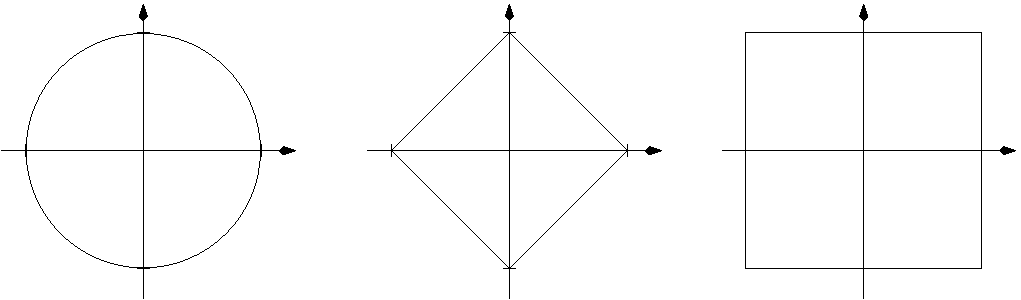
\includegraphics[width=0.75\textwidth]{images/norms.pdf}
%\caption{Unit spheres for the $2$-norm, $1$-norm and $\infty$-norm.}
\end{figure}
\end{center}
The unit sphere with respect to the $2$-norm in $\R^n$ is usually denoted by $S^{n-1}$.

The $1$-, $2$- and $\infty$-norms are equivalent, in the sense that they can be bounded in terms of each other. In particular,
\begin{equation}\label{eq:normineq}\tag{3}
 \norm{\vct{x}}_\infty \leq \norm{\vct{x}}_2\leq \sqrt{n}\norm{\vct{x}}_\infty, \quad \norm{\vct{x}}_\infty \leq \norm{\vct{x}}_1\leq n\norm{\vct{x}}_\infty.
\end{equation}

The inner product and the $2$-norm are related the \marginpar{\textbf{Cauchy-Schwarz}}\textbf{Cauchy-Schwarz} inequality,
\begin{equation*}
 |\ip{\vct{x}}{\vct{y}}| \leq \norm{\vct{x}}_2\norm{\vct{y}}_2,
\end{equation*}
with equality if and only if $\vct{x}$ and $\vct{y}$ are linearly dependent. As a consequence of the Cauchy-Schwarz inequality we get
\begin{equation*}
 -1\leq \frac{\ip{\vct{x}}{\vct{y}}}{\norm{\vct{x}}_2\norm{\vct{y}}_2}\leq 1.
\end{equation*}
The \strictpagecheck\marginpar{\textbf{angle}}\textbf{angle} between vectors $\vct{x}$ and $\vct{y}$ is the number $\theta\in [0,2\pi)$ such that
\marginparmargin{outer}
\begin{equation*}
 \cos(\theta) = \frac{\ip{\vct{x}}{\vct{y}}}{\norm{\vct{x}}_2\norm{\vct{y}}_2}.
\end{equation*}
If $\vct{x}$ and $\vct{y}$ are orthogonal, then $\cos(\theta)=0$ and $\theta\in \{\pi/2,3\pi/2\}$.

Norms are an important device to measure the size of vectors. In order to measure the amount by which a linear transformation (matrix) distorts vectors, we need the concept of
\strictpagecheck\marginpar{\textbf{matrix norm}}\textbf{matrix norms}. A matrix norm is a function on the set of matrices that is a norm when considering a matrix as a vector, and in addition satisfies the condition\marginparmargin{outer}
\begin{equation*}
 \norm{\mtx{A}\mtx{B}}\leq \norm{\mtx{A}}\norm{\mtx{B}}.
\end{equation*}
The most important examples are given by the \marginpar{\textbf{operator norm}}\textbf{operator norms}. Given a vector norm $\norm{\vct{x}}$, the associated matrix norm is defined as
\begin{equation*}
 \norm{\mtx{A}} = \max_{\vct{x}\neq \zerovct} \frac{\norm{\mtx{A}\vct{x}}}{\norm{\vct{x}}} = \max_{\vct{x}\colon \norm{\vct{x}}\leq 1} \norm{\mtx{A}\vct{x}}.
\end{equation*}
The matrix norms $\norm{\mtx{A}}_1, \norm{\mtx{A}}_2, \norm{\mtx{A}}_\infty$ are the operator norms that arise when using the $1$-, $2$- and $\infty$-norms. They can conveniently characterized as follows
\begin{itemize}
 \item $\norm{\mtx{A}}_1 = \max_{j} \sum_{i=1}^n |a_{ij}|$;
 \item $\norm{\mtx{A}}_\infty = \max_{i} \sum_{j=1}^n |a_{ij}|$;
 \item $\norm{\mtx{A}}_2 = \sqrt{\lambda_{\mathrm{max}}(\mtx{A}^{\trans}\mtx{A})}$.
\end{itemize}
Here, $\lambda_{\mathrm{max}}$ denotes the largest eigenvalue of the symmetric matrix $\mtx{A}^{\trans}\mtx{A}$. If $\mtx{A}$ is symmetric, then $\mtx{A}^{\trans}\mtx{A}=\mtx{A}^2$, and the eigenvalues of $\mtx{A}^2$ are the squares of the eigenvalues of $\mtx{A}$. It follows that for symmetric $\mtx{A}$, $\norm{\mtx{A}}_2 = \lambda_{\mathrm{max}}(\mtx{A})$.

\begin{example}
Let
\begin{equation*}
\mtx{A} = \begin{pmatrix}
1 & -2\\
-2 & 1
\end{pmatrix}.
\end{equation*}
Then $\norm{\mtx{A}}_1 = \norm{\mtx{A}}_{\infty} = 3$ and $\norm{\mtx{A}}_2 = 3$.
\end{example}

A special case is the \marginpar{\textbf{dual norm}}\textbf{dual norm} of a vector norm:
to a given norm is defined as
\begin{equation*}
 \norm{\vct{x}}^* = \max_{\vct{y}\colon \norm{\vct{y}}\leq 1} \ip{\vct{x}}{\vct{y}}.
\end{equation*}
This is the operator norm of $\vct{x}^{\trans}$, considered as a $1\times d$ matrix. The dual of the dual norm is the norm itself.
The dual norm of the $2$-norm is again the $2$-norm, while the $1$-norm and the $\infty$-norm are dual to each other.

In addition to the operator norms, an important matrix norm is the \marginpar{\textbf{Frobenius norm}}\textbf{Frobenius norm} of a matrix $\mtx{A}\in \R^{n\times n}$, 
\begin{equation*}
 \norm{\mtx{A}}_{F} = \sqrt{\sum_{i,j=1}^n a_{ij}^2}.
\end{equation*}
This is just the $2$-norm of $\mtx{A}$ interpreted as a vector in $\R^{n^2}$. The $2$-norm and the Frobenius norm have the important property of being \marginpar{\textbf{orthogonal invariant}}\textbf{orthogonal invariant},
which means that for any $\mtx{Q}\in O(n)$,
\begin{equation*}
 \norm{\mtx{Q}\mtx{A}}_2 = \norm{\mtx{A}\mtx{Q}}_2 = \norm{\mtx{A}}_2, \quad \norm{\mtx{Q}\mtx{A}}_F = \norm{\mtx{A}\mtx{Q}}_F = \norm{\mtx{A}}_F.
\end{equation*}
Orthogonal invariance allows to simplify a matrix without changing the norm.

\subsection{Positive semidefinite matrices}
If $\mtx{A}\in \Sym^n$ is a symmetric matrix and $\vct{u}\in \R^n$ an eigenvector with $\norm{u}_2=1$ and corresponding eigenvalue $\lambda$, then $
 \vct{u}^{\trans}\mtx{A}\vct{u} = \lambda \vct{u}^{\trans}\vct{u} = \lambda$.
In particular, the largest and smallest values of an eigenvalue are given by
\begin{equation*}
 \lambda_1 = \max_{\vct{u}\colon \norm{\vct{u}}_2=1} \vct{u}^{\trans}\mtx{A}\vct{u}, \quad \lambda_n = \min_{\vct{u}\colon \norm{\vct{u}}_2=1} \vct{u}^{\trans}\mtx{A}\vct{u}.
\end{equation*}
A symmetric matrix $\mtx{A}$ is called \marginpar{\textbf{positive (semi)definite}}\textbf{positive semidefinite}, written $\mtx{A}\succeq \zerovct$, if for all non-zero $\vct{x}\in \R^n$, $\vct{x}^{\trans}\mtx{A}\vct{x}\geq 0$, and \textbf{positive definite}, written $\mtx{A}\succ \zerovct$, if $\vct{x}^{\trans}\mtx{A}\vct{x}>0$ for all $\vct{x}\neq \zerovct$. Equivalently, a symmetric matrix is positive semidefinite if all its eigenvalues are non-negative, and positive definite if they are all positive.
The set of positive semidefinite symmetric matrices in $\R^{n\times n}$ is denoted by $\SDP^n$, while the set of positive definite matrices is $\Sym_{++}^n$. 

\marginparmargin{outer}
An \marginpar{\textbf{inner product}}\textbf{inner product} (or scalar product) on $\R^{n\times n}$ is a function 
\begin{equation*}
 \ip{\cdot}{\cdot}\colon \R^n\times \R^n \to \R, \quad (\vct{x},\vct{y}) \mapsto \ip{\vct{x}}{\vct{y}}
\end{equation*}
that is bilinear (linear in each of the two arguments), symmetric ($\ip{\vct{x}}{\vct{y}}=\ip{\vct{y}}{\vct{x}}$), and satisfies $\ip{\vct{x}}{\vct{x}}\geq 0$, with $\ip{\vct{x}}{\vct{x}}=0$ if and only if $\vct{x}=\zerovct$. The standard inner product $\ip{\vct{x}}{\vct{y}}=\vct{x}^{\trans}\vct{y}$ is an example, and the notation $\ip{\cdot}{\cdot}$ usually refers to this product. More generally, every matrix $\mtx{A}\in \Sym_{++}^n$ defines an inner product by
\begin{equation*}
 \ip{\vct{x}}{\vct{y}}_{\mtx{A}} := \ip{\vct{x}}{\mtx{A}\vct{y}} = \vct{x}^{\trans}\mtx{A}\vct{y}.
\end{equation*}
The associated norm is $\norm{\vct{x}}_{\mtx{A}}=\sqrt{\ip{\vct{x}}{\vct{x}}_{\mtx{A}}}$. The unit sphere with respect to this norm,
\begin{equation*}
 E = \{\vct{x}\in \R^n \mid \vct{x}^{\trans}\mtx{A}\vct{x}=1\},
\end{equation*}
is an \marginpar{\textbf{ellipsoid}}\textbf{ellipsoid}, where the $2$-norms of the largest and smallest axes are the largest and smallest eigenvalues of $\mtx{A}^{-1}$. 

\subsection{Matrix decompositions} Matrices can be represented as products of simpler matrices. Important examples are:
\marginparmargin{outer}
\begin{enumerate}
 \item \marginpar{\textbf{QR}}\textbf{$QR$ decomposition}. A matrix $\mtx{A}\in \R^{m\times n}$ can be written as
 \begin{equation*}
  \mtx{A} = \mtx{Q}\mtx{R},
 \end{equation*}
where $\mtx{Q}\in \R^{m\times m}$ is an orthogonal, and $\mtx{R}\in \R^{m\times n}$ an upper triangular matrix. Gram-Schmidt orthogonalisation produces such a decomposition.
 \item \marginpar{\textbf{LU}}\textbf{$LU$ decomposition}. A square matrix $\mtx{A}\in \R^{n\times n}$ can be written as
 \begin{equation*}
  \mtx{A} = \mtx{L}\mtx{U}
 \end{equation*}
where $\mtx{L}\in \R^{n\times n}$ is a lower triangular, and $\mtx{U}\in \R^{n\times n}$ an upper triangular matrix. Gaussian eliminations produces such a decomposition.
 \item \marginpar{\textbf{Symmetric\\ eigenvalue\\ decomposition}}\textbf{Symmetric eigenvalue decomposition}. A symmetric matrix $\mtx{A}\in \Sym^n$ can be written as
 \begin{equation*}
  \mtx{A} = \mtx{Q}\mtx{\Lambda} \mtx{Q}^{\trans},
 \end{equation*}
where $\mtx{Q}$ is an orthogonal matrix, with the eigenvectors as rows, and $\mtx{\Lambda}$ a {\em diagonal} matrix with the eigenvalues on the diagonal.
\item \marginpar{\textbf{Cholesky}}\textbf{Cholesky decomposition}. A positive definite symmetric matrix $\mtx{A}\in \Sym_{++}^n$ can be factored as
\begin{equation*}
\mtx{A} = \mtx{L}\mtx{L}^{\trans},
\end{equation*}
with $\mtx{L}\in \R^{n\times n}$ lower-triangular and with strictly positive diagonal entries.
\end{enumerate}

One of the most powerful matrix decompositions is the \marginpar{\textbf{SVD}}\textbf{singular value decomposition} (SVD). It states that any $m\times n$ matrix $\mtx{A}$ can be written as
\begin{equation*}
 \mtx{A} = \mtx{U}\mtx{\Sigma}\mtx{V}^{\trans},
\end{equation*}
where $\mtx{U}$ is a $m\times m$ orthogonal matrix, $\mtx{V}$ an $n\times n$ orthogonal matrix, and $\mtx{\Sigma}$ is a diagonal matrix with the \marginpar{\textbf{singular value}}\textbf{singular values} $\sigma_1\geq \cdots\geq \sigma_{\min\{m,n\}}$ on the diagonal. The singular values are the square roots of the eigenvalues of $\mtx{A}^{\trans}\mtx{A}$. The singular values are related to the matrix $2$-norm and Frobenius norm of $\mtx{A}\in \R^{n\times n}$ as follows:
\begin{equation*}
  \norm{\mtx{A}}_2 = \sigma_1(\mtx{A}), \quad \norm{\mtx{A}}_F = \sqrt{\sum_{i=1}^n \sigma_i^2(\mtx{A})}. 
\end{equation*}
If $\mtx{A}$ is symmetric, the singular values are the absolute values of the eigenvalues of $\mtx{A}$.

Matrix decompositions can help reduce a problem into one involving simpler (orthogonal, triangular) matrices. For example, to solve $\mtx{A}\vct{x}=\vct{b}$, one can first compute $\mtx{A}=\mtx{Q}\mtx{R}$, solve the simpler system of equations $\mtx{Q}\vct{y}=\vct{b}$ by computing $\vct{y}=\mtx{Q}^{\trans}\vct{b}$, and then solve the triangular system $\mtx{R}\vct{x}=\vct{y}$ by back-substitution. 

\begin{example}
Consider the matrix $
  \begin{pmatrix}
    2 & -1\\ -1 & 2
  \end{pmatrix}$.
The $QR$ decomposition is
\begin{equation*}
\mtx{Q} = \frac{1}{\sqrt{5}}\begin{pmatrix}
-2 & 1\\
1 & 2
\end{pmatrix}, \quad
\mtx{R} = \frac{1}{\sqrt{5}}\begin{pmatrix}
-5 & 4\\
0 & 3
\end{pmatrix},
\end{equation*}
the $LU$ decomposition is
\begin{equation*}
\mtx{L} = \begin{pmatrix}
1 & 0\\
-1/2 & 1
\end{pmatrix}, \quad
\mtx{U} = \begin{pmatrix}
  2 & -1\\
  0 & 3/2
\end{pmatrix},
\end{equation*}
the symmetric eigenvalue decomposition and the SVD are given by
\begin{equation*}
 \mtx{\Lambda} = \mtx{\Sigma} = \begin{pmatrix}
 3 & 0\\
 0 & 1
 \end{pmatrix}, \quad
 \mtx{Q} = \mtx{U} = \mtx{V} = \begin{pmatrix}
 \cos(\pi/4) & \sin(\pi/4)\\
 -\sin(\pi/4) & \cos(\pi/4)
 \end{pmatrix},
\end{equation*}
and the Cholesky decomposition is given by
\begin{equation*}
\mtx{L} = \frac{1}{\sqrt{2}}\begin{pmatrix}
2 & 0\\
-1 & \sqrt{3}
\end{pmatrix}.
\end{equation*}
The eigenvalue decomposition shows how to visualize the ellipse $\{\mtx{A}\vct{x} \mid \norm{\vct{x}}_2=1\}$: 
\begin{figure}[ht!]
\centering
\begin{tikzpicture}[thick,rotate=45,scale=0.4]
\filldraw[color=black, fill=blue!5, very thick, rotate=0](0,0) ellipse (3 and 1);

%\node (A1) at (3,0)  [label=180:$\vct{x}$] {};
%\node (A2) at (1,0)   [label=0:$\vct{y}$] {};
\filldraw[black, rotate=0] (3,0) circle (2pt);
\filldraw[black, rotate=0] (0,1) circle (2pt);

\draw[color=blue,thick,->] (0,0) -- (3,0);
\draw[color=blue,thick,->] (0,0) -- (0,1);
\end{tikzpicture}
\end{figure}

Applying the transformation $\mtx{A}\vct{x} = \mtx{Q}\mtx{\Lambda}\mtx{Q}^{\trans}\vct{x}$ corresponds to rotating the vector $\vct{x}$ clockwise by an angle of $\pi/4$, then stretching by a factor of $3$ in the $x$-direction, and then rotating back.
\end{example}

\section{Calculus}
\setcounter{figure}{0}
We write $C([a,b])=C^0([a,b])$ for the set of continuous functions on an interval $[a,b]$, and for $k\geq 1$ we write $C^k([a,b])$ for the set of functions continuous on $[a,b]$, and whose first $k$ derivatives $f',\dots,f^{(k)}$ exist and are continuous on $(a,b)$. In the above definition we allow $a=-\infty$ or $b=\infty$. If $a,b\in \R$, then any function $f\in C([a,b])$ is bounded. The \strictpagecheck\marginpar{\textbf{infimum}}\textbf{infimum} (largest lower bound) and \marginpar{\textbf{supremum}}\textbf{supremum} (smallest upper bound) of a function $f$ on an interval $[a,b]$ are defined as
\begin{align*}
 \inf_{x\in [a,b]} f(x) &= \max\{y\in \R \mid \forall x\in [a,b], f(x)\geq y\},\\
  \sup_{x\in [a,b]} f(x) &= \min\{y\in\R \mid \forall x\in [a,b], f(x)\leq y\}.
\end{align*}
Again, we allow the ``values'' $-\infty$ and $\infty$. If the infimum is attained (i.e., there exists $x^*$ such that $f(x^*) = \inf_{x\in [a,b]} f(x)$), then we write $\min_{x\in [a,b]}f(x)$, and similarly $\max$ if the supremum is attained. Any $f\in C([a,b])$ for $a,b\in \R$ attains its infimum and supremum on $[a,b]$.

Three important concepts are the \textbf{Intermediate Value Theorem}, the \textbf{Mean Value Theorem}, and the \textbf{Taylor expansion}. 

\begin{theorem*}[\textbf{Intermediate Value Theorem}]
\strictpagecheck
\marginpar{\textbf{Intermediate\\ Value Theorem}}If $f\in C([a,b])$ and if $y$ satisfies
\begin{equation*}
\inf_{x\in [a,b]} f(x)\leq y\leq \sup_{x\in [a,b]} f(x),
\end{equation*}
then there exists $\xi \in [a,b]$ such that $f(\xi)=y$. In particular, the infimum and supremum are attained.
\end{theorem*}
\marginparmargin{outer}

\begin{theorem*}[\textbf{Mean Value Theorem}]
\marginpar{\textbf{Mean Value Theorem}}
Let $f\in C^1([a,b])$ and let $x,x_0\in (a,b)$ with $x\neq x_0$. 
Then there exists a number $\xi\in (x_0,x)$ (or $(x,x_0)$ if $x<x_0$) such that
\begin{equation*}
  f(x) = f(x_0)+f'(\xi)(x-x_0).
\end{equation*}
This can also be written as
\begin{equation*}
  f'(\xi) = \frac{f(x)-f(x_0)}{x-x_0}.
\end{equation*}
\end{theorem*}

\begin{figure}[h!]
\centering
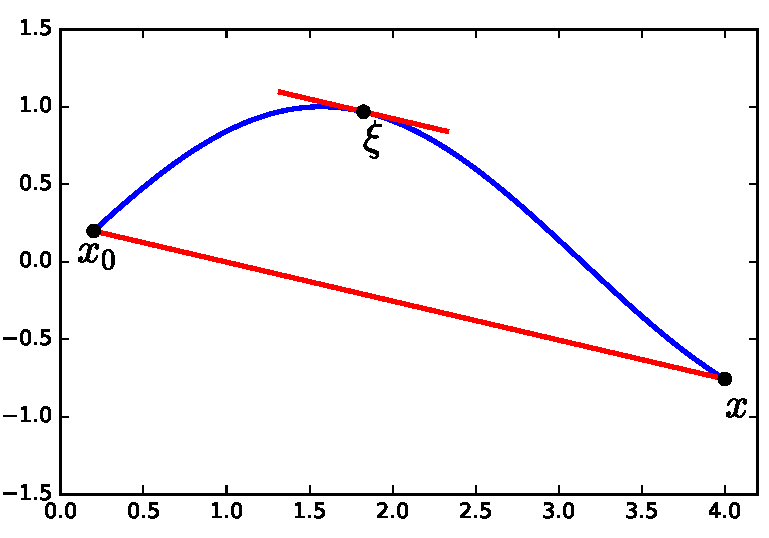
\includegraphics[width=0.4\textwidth]{images/mvt.pdf}
\caption{\small MVT: there exists a point at which the slope (derivative) is the same as that of the secant connecting $(x_0,f(x_0))$ and $(x,f(x))$.}
\end{figure}

The Mean Value Theorem is a special case of the Taylor expansion.

\begin{theorem*}[\textbf{Taylor expansion}]
\marginpar{\textbf{Taylor series}}
Let $f\in C^{(n)}([a,b])$ and let $x,x_0\in(a,b)$ with $x\neq x_0$. Then
there exists $\xi\in (x,x_0)$ (or $(x,x_0)$ if $x<x_0$) such that
\begin{align*}
  f(x) = f(x_0)&+f'(x_0)(x-x_0)+\frac{1}{2}f''(x_0)(x-x_0)^2+\cdots \\
   &+\frac{f^{(n)}(x_0)}{n!}(x-x_0)^n + \frac{f^{(n+1)}(\xi)}{(n+1)!}(x-x_0)^{n+1}
\end{align*}
\end{theorem*}

The first $(n+1)$ terms of the above sum can be seen as an approximation to the function $f$ that becomes more accurate as $n$ increases. 
The last term is known as the {\em truncation error} in numerical approximation.

As an example, consider the Taylor expansion of the sine function at $x_0=0$,
\begin{equation*}
\sin(x) = x-\frac{x^3}{3!}+\frac{x^5}{5!}-\cdots
\end{equation*}

The Taylor approximation to different orders is illustrated in the following figure.

\begin{center}
\begin{figure}[h!]
\centering
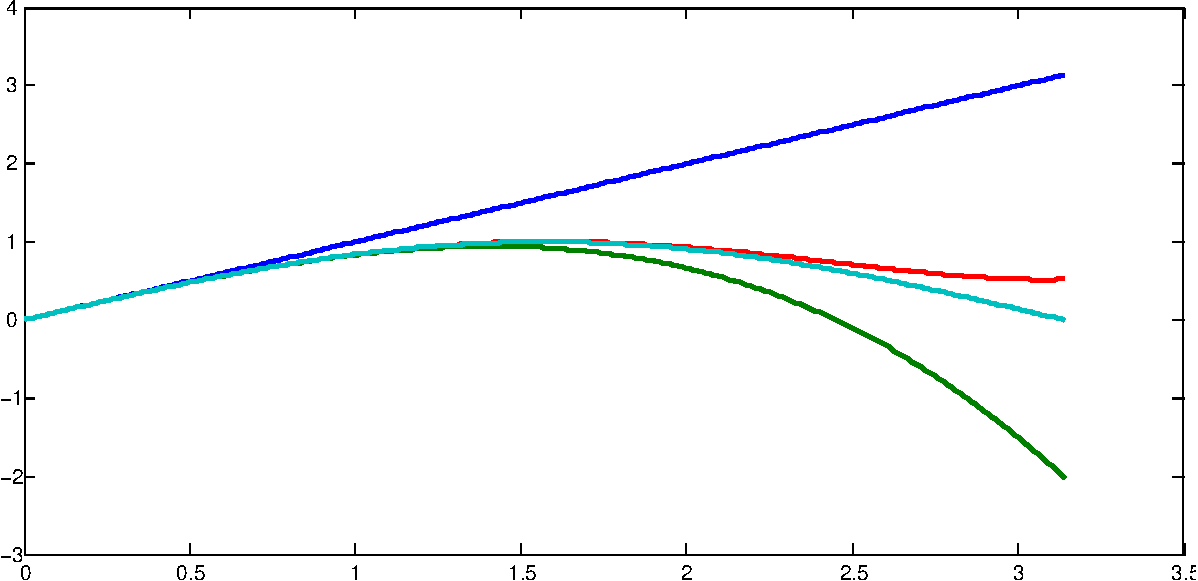
\includegraphics[width=0.5\textwidth]{images/sine-crop.pdf}
\caption{\small Taylor expansion of $\sin(x)$.}
\end{figure}
\end{center}

A special case is of the Mean Value Theorem is \textbf{Rolle's Theorem}.

\begin{theorem*}[Rolle's Theorem]
\marginpar{\textbf{Rolle's Theorem}}
Let $f\in C^1([a,b])$ with $f(a) = f(b)$. Then there exists 
a number $\xi\in (a,b)$ such that $f'(\xi) = 0$.
\end{theorem*}

\begin{figure}[h!]
\centering
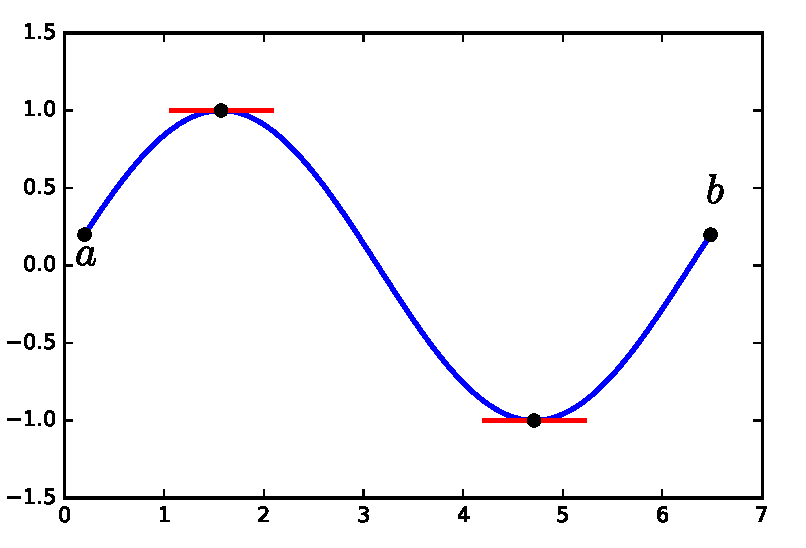
\includegraphics[width=0.5\textwidth]{images/rolle.pdf}
\caption{\small Rolle's Theorem: there exist points with ``flat" slope (derivative zero).}
\end{figure}

The intuition is that if you walk across mountains and arrive at a point with the same elevation as where you started, then there must be places on the way where the slope is $0$, that is, a local maximum or minimum. Of importance is also the following variant of the the Mean Value Theorem.

\begin{theorem*}[\textbf{Integral Mean Value Theorem}]
\marginpar{\textbf{Integral MVT}}Let $f,g\in C([a,b])$ and assume that $f(x)$ does not change sign on $[a,b]$. Then
there exists a $\xi\in (a,b)$ such that
\begin{equation*}
  \int_a^b f(x)g(x) \ dx = g(\xi) \int_a^b f(x) \ dx.
\end{equation*}
\end{theorem*}

\subsection{Topology}
\strictpagecheck
The \marginpar{\textbf{open ball}}\textbf{open ball} of radius $\e$ around $\vct{p}\in \R^n$ is defined as
\begin{equation*}
 B^n(\vct{p},\e) = \{\vct{x} \mid \norm{\vct{x}-\vct{p}}_2<\e\}.
\end{equation*}
We write $B^n:=B^n(\zerovct,1)$ for the (open) \textbf{unit ball}.
A subset $U\subseteq \R^n$ is called \marginpar{\textbf{open and closed set}}\textbf{open} if for every $p\in U$ there exists an $\e>0$ such that $B(\vct{p},\e)\subset U$. A set $C$ is \textbf{closed} if $\overline{C}=\R^n\backslash C$ is open. 
The \marginpar{\textbf{closure}, \textbf{boundary},\\ \textbf{interior}}\textbf{closure} $\cl S$ of a set $S\subseteq \R^n$ is the intersection of all closed sets containing $S$, while the \textbf{interior} $\inter S$ is the union of all open sets contained in $S$. 
The \textbf{boundary} of $S$ is defined as $\bd S = \cl S\backslash \inter S$. For example, the boundary of the open unit ball is the \marginpar{\textbf{unit sphere, ball}}\textbf{unit sphere}
\begin{equation*}
 \bd B^n = S^{n-1} = \{\vct{x}\in \R^n \mid \norm{\vct{x}}_2 = 1\}.
\end{equation*}
The superscript $n-1$ refers to the fact that this set is a manifold of dimension $n-1$. A \strictpagecheck\marginpar{\textbf{neighbourhood}}\textbf{neighbourhood} $N$ of a point $\vct{x}\in \R^n$ is a set such that there exists an open set $U$ with $\vct{x}\in U\subseteq N$. An \textbf{open neighbourhood} is a neighbourhood that is open. 
\marginparmargin{outer}Note that if $U_1\subseteq \R^n$ and $U_2\subseteq \R^m$ are open sets, then the product $U_1\times U_2 \subseteq \R^{n+m}$ is also open. 

Any subset $S\subseteq \R^n$ inherits a topological structure from $\R^n$, where the open sets in $S$ are the sets of the form $U\cap S$, with $U\subseteq \R^n$ open. 
If a set $S$ is contained in a lower-dimensional linear subspace $V\subset \R^n$, say, with $\dim V=k<n$, then $S$ is always closed. However, it can be open {\em relative to its linear span},
\begin{equation*}
 \mathrm{span}(S) = \left\{\sum_{i=1}^k \lambda_i \vct{x}_i \mid \lambda_1,\dots,\lambda_k\in \R, \vct{x}_1,\dots,\vct{x}_k\in S\right\}.
\end{equation*}
We call a set $S$ \marginpar{\textbf{relatively open},\\\textbf{relatively closed}}\textbf{relatively open} or \textbf{relatively closed} if it is open or closed in the induced topology on $\mathrm{span}(S)$. Another way of defining this notion goes as follows.
Let $\{\vct{b}_1,\dots,\vct{b}_k\}$ be an orthonormal basis of $\mathrm{span}(S)$, with $\mtx{B}=(\vct{b}_1,\dots,\vct{b}_k)$, and consider the map
\begin{equation*}
 \varphi_{\vct{B}}\colon \R^k \to \mathrm{span}(S),\quad \varphi_{\mtx{B}}(\vct{x})=\sum_{i=1}^k x_i \vct{b}_i.
\end{equation*}
Then a set $S$ is relatively open or relatively closed if the preimage 
\begin{equation*}
\varphi_{\vct{B}}^{-1}(S) = \{\vct{x} \mid \varphi_{\mtx{B}}(\vct{x})\in S\}
\end{equation*}
is open or closed in $\R^k$. Based on these notions, one defines the \marginpar{\textbf{relative closure},\\\textbf{relative interior}}\textbf{relative closure} $\relcl S$ and \textbf{relative interior} $\relint S$ just as before.

\begin{figure}[h!]
\centering
\begin{tikzpicture}[scale=2.5,tdplot_main_coords]

%set up some coordinates 
%-----------------------
\coordinate (O) at (0,0,0);

%draw figure contents
%--------------------
\filldraw[fill=red!20, draw=none] (O) -- (0.8,0,0) -- (0.8,0.8,0) -- (0,0.8,0) -- cycle; 

%draw the main coordinate system axes
\draw[thin,->] (O) -- (1,0,0) node[anchor=north east]{$x$};
\draw[thin,->] (O) -- (0,1,0) node[anchor=north west]{$y$};
\draw[thin,->] (O) -- (0,0,0.5) node[anchor=south]{$z$};

\tikzset{yxplane/.style={canvas is yx plane at z=#1,very thin}}
\begin{scope}[yxplane=0]
   \draw[fill=blue!20, dashed, thick] (0.4,0.4) circle[radius=0.2] ;
 \end{scope}
%draw points v_1 and v_2
\end{tikzpicture}
\caption{The disk without boundary on the $xy$-plane is relatively open, and is the relative interior of the disk with boundary.} 
\end{figure}

A subset $S\subseteq \R^n$ is \marginpar{\textbf{bounded}}\textbf{bounded} if there exists number $M>0$ such that $\norm{\vct{x}}_2<M$ for all $\vct{x}\in S$. Invoking the equivalence of norms~\eqref{eq:normineq} one sees that this definition does not depend on the norm chosen.
A set $K\subseteq \R^n$ is called \marginpar{\textbf{compact}}\textbf{compact} if it is closed and bounded. Equivalently, every cover of $K$ with open sets contains a finite subcover.  
A function $f\colon \R^n\to \R^m$ is \marginpar{\textbf{continuous}}\textbf{continuous} if for every open set $U\subset \R^m$,
\begin{equation*}
 f^{-1}(U) := \{\vct{x}\in \R^n\mid f(\vct{x})\in U\}
\end{equation*}
is an open subset of $\R^n$. 
A function defined on a subset $S\subseteq \R^n$ is said to be continuous if it is continuous on the induced topology. The set of continuous functions $f\colon S\to \R^m$ is denoted by $C(S,\R^m)=C^0(S,\R^m)$.
If $f\in C(K,\R)$, where $K$ is compact, then $f$ is bounded, and attains its infimum and supremum there: there exist $\vct{x}_*,\vct{x}^*\in K$ such that
\begin{equation*}
 \inf_{\vct{x}\in K} f(\vct{x}) = f(\vct{x}_*), \quad \sup_{\vct{x}\in K} f(\vct{x}) = f(\vct{x}^*).
\end{equation*}
A weaker notion is that of a \marginpar{\textbf{Lipschitz}}\textbf{Lipschitz continuous} function. A function $f\colon S\to \R^m$ is called Lipschitz continuous with Lipschitz constant $L>0$, if for all $\vct{x},\vct{y}\in S$,
\begin{equation*}
 \norm{f(\vct{x})-f(\vct{y})}_2 \leq L\norm{\vct{x}-\vct{y}}_2.
\end{equation*}

\strictpagecheck
Notions about continuity of functions can be conveniently stated in terms of sequences.
A \marginpar{\textbf{sequence}}\textbf{sequence} of points $\{\vct{x}_k\}_{k\in \N}\subset \R^n$ (for short, $\{\vct{x}_k\}$) 
\marginpar{\textbf{convergence}}\textbf{converges} to $\vct{x}\in \R^n$ as $k\to \infty$ with respect to a norm $\norm{\cdot}$, written $\vct{x}_k\to \vct{x}$, if the sequence of numbers $\norm{\vct{x}_k-\vct{x}}$ converges to $0$,
\begin{equation*}
 \lim_{k\to \infty} \norm{\vct{x}_k-\vct{x}}=0.
\end{equation*}
Formally, this means that for every $\e>0$ there exists an index $k_0$, such that for all $k>k_0$, $\norm{\vct{x}_k-\vct{x}}<\e$. From the equivalence of norms~\eqref{eq:normineq} it follows that if a sequence converges with respect to one norm, it also converges with respect to the other norms. 

A \marginpar{\textbf{subsequence}}\textbf{subsequence} of a sequence $\{\vct{x}_k\}$ is an infinite subset of $S$.
A \marginpar{\textbf{limit point}}\textbf{limit point} for a sequence $S=\{\vct{x}_k\}$ is a point $\vct{x}$ that is the limit of an subsequence of $S$. Formally, for every $\e>0$ there exists a $k_0$ such that $\norm{\vct{x}_k-\vct{x}}<\e$ {\em for some} $k>k_0$. A sequence $\{\vct{x}_k\}$ is called a \marginpar{\textbf{Cauchy sequence}}\textbf{Cauchy sequence} if for every $\e>0$ there exists an index $k_0>0$, such that for all $k,\ell>k_0$, $\norm{\vct{x}_k-\vct{x}_{\ell}}_2<\e$. The vector space $\R^n$ with the $2$-norm (or any other norm) is a \marginpar{\textbf{Banach space}}\textbf{Banach space}, which means that every Cauchy sequence contains a convergent subsequence.

All the topological notions discussed earlier have an interpretation in terms of sequences and limits:
\begin{enumerate}
\item A set $C$ is closed if and only if for every sequence $\{x_k\}\subset C$, all limit points are in $C$; 
\item The closure of a set $S$ is the set of all limit points of sequences in $S$;
\item A set $K$ is compact, if and only if every sequence of points $\{x_k\}$ in $K$ has a limit point in $K$.
\end{enumerate}

Given a function $f\colon \Omega \to \R^m$, where $\Omega\subseteq \R^n$, and $\vct{x}\in \Omega$, then $f$ is \marginpar{\textbf{continuous at $\vct{x}^*$}}\textbf{continuous at $\vct{x}^*$} if 
\begin{equation*}
 \lim_{\vct{x}\to \vct{x}^*} f(\vct{x}) = f(\vct{x}^*).
\end{equation*}
Formally, for every $\e>0$ there exists a $\delta>0$ such that whenever $\norm{\vct{x}-\vct{x}^*}<\delta$, $\norm{f(\vct{x})-f(\vct{x}^*)}<\e$.
This means that for every sequence of points $\{\vct{x}_k\}$ with $\lim_{k\to \infty}\vct{x}_k=\vct{x}^*$, the sequence $f(\vct{x}_k)\to f(\vct{x}^*)$ as $k\to \infty$ with respect to some norm on $\R^m$.\marginparmargin{outer}

\subsection{Differentiable functions}
A function $f\colon \R^n\to \R^m$ is called (Fr\'echet) \marginpar{\textbf{differentiable}}\textbf{differentiable} at $\vct{x}_0\in \R^n$ if there exists a linear map $\mtx{J}f(\vct{x}_0)\colon \R^n \to \R^m$, such that
\begin{equation*}
 \lim_{\vct{h}\to \zerovct}\frac{\norm{f(\vct{x}_0+\vct{h})-f(\vct{x}_0)-\mtx{J}f(\vct{x}_0)\vct{h}}_2}{\norm{\vct{h}}_2}=0.
\end{equation*}
A function is differentiable on an open subset $U\subseteq \R^n$ if it is differentiable at every $\vct{x}\in U$.
If $f(\vct{x})=(f_1(\vct{x}),\dots,f_m(\vct{x}))^{\trans}$ is differentiable, then all the partial derivatives exist, and $\mtx{J}f(\vct{x}_0)$ is represented by the \marginpar{\textbf{Jacobian}}\textbf{Jacobian matrix}
\begin{equation*}
 \mtx{J}f(\vct{x}_0) = \begin{pmatrix}
            \frac{\partial f_1}{\partial x_1} & \cdots & \frac{\partial f_1}{\partial x_n}\\
            \vdots & \ddots & \vdots\\
            \frac{\partial f_m}{\partial x_1} & \cdots & \frac{\partial f_m}{\partial x_n}
           \end{pmatrix},
\end{equation*}
where the partial derivatives are evaluated at $\vct{x}_0$. If all the partial derivatives exist and are continuous in a neighbourhood of $\vct{x}_0$ (called \marginpar{\textbf{continuously\\ differentiable}}\textbf{continuously differentiable}), then $f$ is differentiable at $\vct{x}_0$.

If $m=1$, then $J(\vct{x}_0)$ is the transpose of the \marginpar{\textbf{gradient}}\textbf{gradient} $\nabla f(\vct{x}_0)$ of $f$ at $\vct{x}_0$,
\begin{equation*}
 \nabla f(\vct{x}_0) = \left(\frac{\partial f}{\partial x_1},\dots,\frac{\partial f}{\partial x_n}\right)^{\top}.
\end{equation*}
The gradient points in the direction in which $f$ increases the most. 

\begin{figure}[ht!]
\centering
\begin{minipage}{0.45\textwidth}
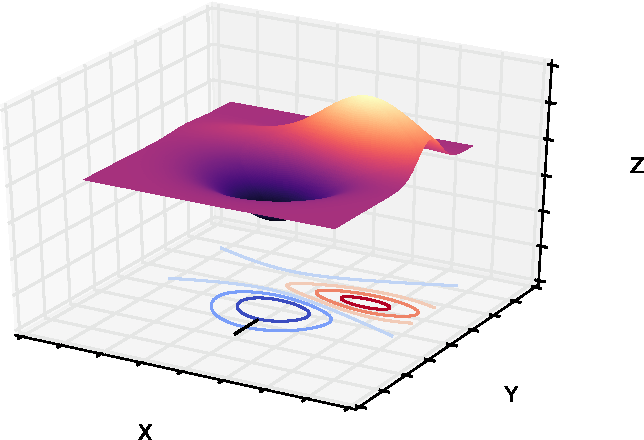
\includegraphics[width=\textwidth]{images/3dsurf.pdf}
\end{minipage}
\begin{minipage}{0.45\textwidth}
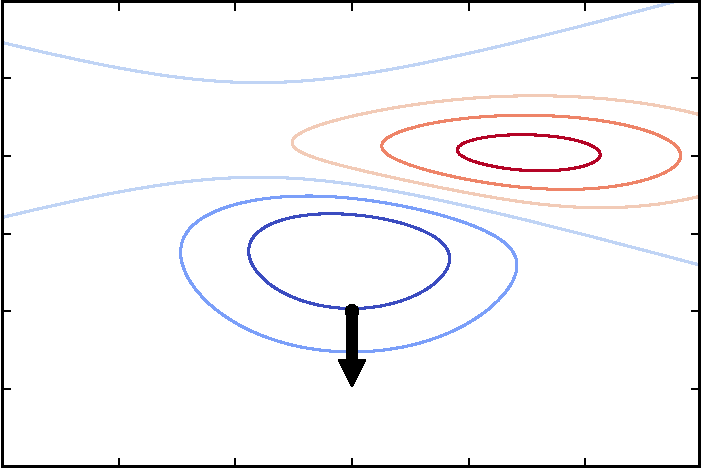
\includegraphics[scale=0.4]{images/contour.pdf}
\end{minipage}
\caption{A surface, level sets, and the gradient}\label{fig:level}
\end{figure}

A convenient way to visualise a function $f\colon \R^2\to \R$ is through \marginpar{\textbf{level set}}\textbf{level sets} $\{\vct{x}\in \R^2 \mid f(\vct{x})=c\}$. For each $c\in \R$, such a level set defines a curve in $\R^2$, the curve on which the function value does not change. The gradient is always orthogonal to the level set, pointing in the direction in which $f$ increases the most (see Figure~\ref{fig:level}).

 If the gradient, considered as a map $\R^n\to \R^n$, is itself differentiable at $\vct{x}_0$, then the Jacobian matrix of the gradient is called the \marginpar{\textbf{Hessian}}\textbf{Hessian matrix}, 
\begin{equation*}
 \nabla^2f(\vct{x}_0) = \begin{pmatrix}
                         \frac{\partial^2f}{\partial x_1\partial x_1} & \cdots & \frac{\partial^2f}{\partial x_1\partial x_n}\\
                         \vdots & \ddots & \vdots\\
                         \frac{\partial^2f}{\partial x_n\partial x_1} & \cdots & \frac{\partial^2f}{\partial x_n\partial x_n}
                        \end{pmatrix}
\end{equation*}
Since
\begin{equation*}
 \frac{\partial^2f}{\partial x_i\partial x_j} = \frac{\partial^2f}{\partial x_j\partial x_i}, 
\end{equation*}
the Hessian is a symmetric matrix.

The \marginpar{\textbf{directional derivative}}\textbf{directional derivative} $D_{\vct{x}_0}f(\vct{x}_0)$ of a function $f\colon \R^n\to \R^m$ in direction $\vct{v}\in \R^n$ at $\vct{x}_0$ is defined as
\begin{equation*}
 D_{\vct{v}}f(\vct{x}_0) = \lim_{h\to 0}\frac{f(\vct{x}_0+h\vct{v})-f(\vct{x}_0)}{h}.
\end{equation*}
In the special case where $\vct{v}=\vct{e}_i$, we obtain the partial derivative with respect to $x_i$,
\begin{equation*}
 \frac{\partial f}{\partial x_i}(\vct{x}_0) = D_{\vct{e}_i}f(\vct{x}_0).
\end{equation*}
If $f\colon \R^n\to \R$ is differentiable with continuous derivative near $\vct{x}_0$, then
\begin{equation*}
 D_{\vct{v}}f(\vct{x}_0) = \nabla f(\vct{x}_0)^{\trans}\vct{v} = \ip{\nabla f(\vct{x}_0)}{\vct{v}}.
\end{equation*}

If $f\colon \R^n\to \R^m$ and $g\colon \R^m\to \R^p$ are differentiable in a neighbourhood of $\vct{x}_0\in \R^n$ and $f(\vct{x}_0)\in \R^m$, respectively, then the composition $h=g\circ f\colon \R^n\to \R^p$ is continuously differentiable in a neighbourhood of $\vct{x}_0$, and the Jacobian matrix is defined by the \marginpar{\textbf{chain rule}}\textbf{chain rule}:
\begin{equation*}
 Jh(\vct{x}_0) = Jg(f(\vct{x}_0))Jf(\vct{x}_0).
\end{equation*}
If $n=1$, then $f\colon \R\to \R^n$ is called a \marginpar{\textbf{curve}}\textbf{curve}, and we write 
\begin{equation*}
 Jf = \frac{\diff{f}}{\diff{t}}=\dot{f}=(\dot{f}_1,\dots,\dot{f}_n)^{\trans}\in \R^n
\end{equation*}
for the derivative of the curve. If $\dot{f}(t_0)=\vct{v}\in \R^n$ and $g\colon \R^n\to \R$, then by the chain rule, the derivative of $g\circ f\colon \R\to \R$ is the directional derivative of $g$ in the direction~$\vct{v}$,
\begin{equation*}
 \frac{\diff{g\circ f}(t_0)}{\diff{t}} = \ip{\nabla g(f(t_0))}{\vct{v}}.
\end{equation*}

Before going on to deal with higher derivative, we state the generalisation of the Mean Value Theorem to higher dimensions.

\begin{theorem*}[Multivariate Mean Value Theorem]
\strictpagecheck\marginpar{\textbf{Multivariate MVT}}
Let $f\in C^1(U)$ for an open set $U$ with $\vct{x}_0,\vct{x}\in U$, $\vct{x}\neq \vct{x}_0$. Then there exists $t\in (0,1)$ such that
\begin{equation*}
  f(\vct{x})-f(\vct{x}_0) = \ip{\nabla f(t\vct{x}+(1-t)\vct{x}_0)}{\vct{x}-\vct{x}_0}.
\end{equation*}
\end{theorem*}
Note that $t\vct{x}+(1-t)\vct{x}_0$ parametrises the line segment connecting $\vct{x}$ and $\vct{x}_0$. 
\marginparmargin{outer}

For a tuple of natural number $\alpha = (\alpha_1,\dots,\alpha_n)$, set $|\alpha|=\sum_{i=1}^n \alpha_i$, and define the higher order partial derivative
\begin{equation*}
 D^\alpha f(\vct{x}) = \frac{\partial^{|\alpha|}f(\vct{x})}{\partial^{\alpha_1}x_1\cdots \partial^{\alpha_n}x_n}.
\end{equation*}
For a set $S\subseteq \R^n$, denote by $C^k(S,\R^m)$ the set of functions $f$ such that all partial derivatives $D^\alpha f$ with $|\alpha|\leq k$ exists and are continuous on $\inter S$. If $m=1$, we write $C^k(S):=C^k(S,\R)$.

Define, for a vector $\vct{x}$ and multi-index $\alpha$,
\begin{equation*}
 \vct{x}^{\alpha} := x_1^{\alpha_1}\cdots x_n^{\alpha_n}.
\end{equation*}
We then have the \marginpar{\textbf{Taylor series}}\textbf{Taylor expansion} around a point $\vct{x}_0$,
\begin{equation*}
 f(\vct{x}) = \sum_{|\alpha|\leq k} D^{\alpha}f(\vct{x}_0)(\vct{x}-\vct{x}_0)^{\alpha} + \sum_{|\alpha|=k} r_\alpha(\vct{x})(\vct{x}-\vct{x}_0)^{\alpha},
\end{equation*}
with $r_\alpha(\vct{x})\to 0$ as $\vct{x}\to \vct{x}_0$.

If a differentiable function $f(\vct{x})$ has a local minimum or maximum at a point $\vct{x}$, then this point satisfies $\nabla f(\vct{x})=0$,
that is, it is a critical point. 
The \marginpar{\textbf{Lagrange multipliers}}\textbf{Lagrange multiplier theorem} says something about local extrema under certain constraints.

\begin{theorem*}[\textbf{Lagrange multipliers}]
Let $\vct{x}^*$ be maximum of $f(\vct{x})$ under the constraint $g(\vct{x})=c$ (that is, a maximum among all points $\vct{x}$ such that $g(\vct{x})=c$). Then there exist a $\lambda\in \R$ 
such that
\begin{equation*}
  \nabla f(\vct{x}^*) = \lambda \nabla g(\vct{x}^*).
\end{equation*}
\end{theorem*}

The \marginpar{\textbf{Lagrangian}}\textbf{Lagrangian} of a function $f(\vct{x})$ with constraint $g(\vct{x})=c$ is the function $\Lambda \colon \R^n\times \R\rightarrow \R$ defined by
\begin{equation*}
  \Lambda(\vct{x},\lambda) = f(\vct{x})-\lambda (g(\vct{x})-c).
\end{equation*}
The Lagrange multiplier theorem then says that if $\vct{x}^*$ is a maximum point of $f(\vct{x})$ under the constraint $g(\vct{x})=c$, then there exists $\lambda\in \R$ such that the pair $(\vct{x}^*,\lambda)$ is
a critical point of the Lagrangian $\Lambda(\vct{x},\lambda)$. 

The \marginpar{\textbf{Implicit Function\\ Theorem}}\textbf{Implicit Function Theorem} is one of the most important results in analysis, and underlies much of differential geometry and physics. 
Let $F\colon \R^{n}\times \R^{m}\to \R^n$ by a function that is continuously differentiable in a neighbourhood of a point $(\vct{x}_0,\vct{y}_0)$, with $\vct{x}_0\in \R^n$ and $\vct{y}_0\in \R^m$. The Jacobian $J_{\vct{x}}(\vct{x}_0,\vct{y}_0)$ with respect to the first set of $n$ coordinates consists of the first $n$ columns of the Jacobian matrix,
\begin{equation*}
 J_{\vct{x}}(\vct{x}_0,\vct{y}_0) = \begin{pmatrix}
                                     \frac{\partial f_1}{\partial x_1}(\vct{x}_0,\vct{y}_0) & \cdots & \frac{\partial f_1}{\partial x_n}(\vct{x}_0,\vct{y}_0)\\
                                     \vdots & \ddots & \vdots\\
                                     \frac{\partial f_m}{\partial x_1}(\vct{x}_0,\vct{y}_0) & \cdots & \frac{\partial f_m}{\partial x_n}(\vct{x}_0,\vct{y}_0)
                                    \end{pmatrix}
\end{equation*}
The interpretation is that we consider $f$ as a function in only the first set of coordinates, with the remaining ones (denoted by $\vct{y}$) considered as parameters.

\begin{theorem*}[\textbf{Implicit Function Theorem}]
Let $f\colon \R^n\times \R^m\to \R^n$ be $k$ times continuously differentiable in an open neighbourhood of $(\vct{x}_0,\vct{y}_0)\in \R^{n}\times \R^m$, and assume that $f(\vct{x}_0,\vct{y}_0) = \zerovct$. Assume further 
that the Jacobian $J_{\vct{x}}f(\vct{x}_0,\vct{y}_0)\in \R^{n\times n}$ in the first $n$ coordinates is {\em non-singular} at $(\vct{x}_0,\vct{y}_0)$. Then there exists an open neighbourhood $\vct{y}_0\in U_{\vct{y}}\subseteq \R^m$, and a function $h\in C^k(U_{\vct{y}},\R^n)$ such that 
\begin{itemize}
 \item $h(\vct{y}_0) = \vct{x}_0$,
\item $f(h(\vct{y}),\vct{y})=0$ for $\vct{y}\in U_{\vct{y}}$.
\end{itemize}
Moreover, the Jacobian of $h$ is given by
\begin{equation*}
 Jh(\vct{y}) = -Jf_{\vct{y}}(h(\vct{y}),\vct{y}) (J_{\vct{x}}f(h(\vct{y}),\vct{y}))^{-1}
\end{equation*}
for all $\vct{y}\in U_{\vct{y}}$.
\end{theorem*}

\begin{example}
 Let $f(x,y)=x^2+y^2-1$ and $(x_0,y_0)=(1,0)$. The Jacobian of $f$ in the first coordinate is
 \begin{equation*}
  \frac{\partial f}{\partial x}(1,0) = 2 \neq 0, 
 \end{equation*}
which is non-singular. Choosing the neighbourhood $U_y=(-1,1)$, the open interval between $-1$ and $1$, we get the function $h\colon U_y\to \R$ as
\begin{equation*}
 h(y) = \sqrt{1-y^2}.
\end{equation*}
This function is defined and differentiable on $(-1,1)$, and satisfies
\begin{equation*}
 f(h(y),y) = h(y)^2+y^2-1 = (1-y^2)+y^2-1 = 0, \quad y\in U_y.
\end{equation*}
The derivative of $h$ can be computed using the chain rule:
\begin{equation*}
 \frac{\diff{f}(h(y),y)}{\diff{y}} = \frac{\partial f}{\partial x}(h(y),y)\frac{\diff{h}}{\diff{y}}(y)+\frac{\partial f}{\partial y}(h(y),y)\frac{\diff{y}}{\diff{y}} 
\end{equation*}
from which we get
\begin{equation*}
 \frac{\diff{h}}{\diff{y}}(y) = -\frac{\partial f}{\partial y}(h(y),y)\left(\frac{\partial f}{\partial x}(h(y),y)\right)^{-1} = -y(1-y^2)^{-3/2}.
\end{equation*}
In this example, the implicit function theorem just gives the usual way of parametrising part of the circle.

\begin{figure}[ht!]
\centering
\begin{tikzpicture}[thick,scale=0.4]
\filldraw[color=black, fill=blue!5, dashed, rotate=0](0,0) circle (3 and 3);

%\node (A1) at (3,0)  [label=180:$\vct{x}$] {};
%\node (A2) at (1,0)   [label=0:$\vct{y}$] {};
\filldraw[black, rotate=0] (3,0) circle (2pt);

\draw[dashed,->] (0,0) -- (4,0);
\draw[dashed,->] (0,0) -- (0,4);
%\draw[very thick,color=blue] (0,-2.9) -- (0,2.9);
\draw [blue,very thick,domain=-89:89] plot ({3*cos(\x)}, {3*sin(\x)});
\node (A1) at (4,0) [label=0:$x$] {};
\node (A2) at (0,4) [label=90:$y$] {};
\end{tikzpicture}
\caption{The blue arc is parametrised by $h(y)=\sqrt{1-y^2}$ for $y\in (-1,1)$.}
\end{figure}

\end{example}

\section{Finite precision arithmetic}
In practical applications, one often cannot simply plug numbers into formulae and get all the exact results. Most numerical data also requires an infinite 
amount of storage (just try to store $\pi$ on a computer!), but a piece of paper or a computer only has limited space. These are some of the reasons that lead us to work with \marginpar{\textbf{approximation}}\textbf{approximations}.

\subsection{Measuring errors}
To measure the quality of approximations, we use the concept of \textbf{relative error}. Given a quantity $x$ and a computed approximation $\hat{x}$, the \marginpar{\textbf{absolute and relative error}}\textbf{absolute error} is given by
\begin{equation*}
  E_{\mathrm{abs}}(\hat{x}) = |x-\hat{x}|,
\end{equation*}
while the {\em relative error} is given as
\begin{equation*}
 E_{\mathrm{rel}}(\hat{x}) = \frac{|x-\hat{x}|}{|x|}.
\end{equation*}
The benefit of working with relative errors is that they are scale invariant. Absolute errors can be meaningless at times: for example, an error of one hour is irrelevant when estimating the age of Stan the Tyrannosaurus Rex at Manchester Museum, but it is crucial when determining the time of a lecture. That is because in the former one hour corresponds to a relative error is of the order $10^{-11}$, while in 
the latter it is of the order $1$.

\subsection{Floating point and significant figures}
The established way of representing real numbers on computers is using \marginpar{\textbf{floating-point}}\textbf{floating-point arithmetic}. In the double precision version of the IEEE standard
for floating-point arithmetic, a number is represented using $64$ bits, where a bit is either $1$ or $0$. A number is written
\begin{equation*}
  x = \pm f \times 2^e,
\end{equation*}
where $f$ is a fraction in $[0,1]$, represented using $52$ bits, and $e$ is the exponent, using $11$ bits, and one bit is for the sign. 
There are largest possible numbers, and there are gaps between representable numbers. The largest
and smallest numbers representable in this form are of the order of $\pm 10^{308}$, enough for most practical purposes. A bigger concern are the gaps, which 
means that the results of many computations almost always have to be rounded to the closest floating-point number. 

When going through calculations without using a computer, we usually use the terminology 
of \marginpar{\textbf{significant figure}}\textbf{significant figures} (s.f.) and work with $4$ significant figures in base 10. 
For example, in base $10$, $\sqrt{3}$ equals $1.732$ to $4$ significant figures. 
To count the number of significant figures in a given number, start with the first
non-zero digit from the left and, moving to the right, count all the
digits thereafter, counting final zeros if they are to the right of
the decimal point. For example, 1.2048, 12.040, 0.012048, 0.0012040
and 1204.0 all have 5 significant figures (s.f.). In rounding or truncation
of a number to $n$ s.f., the original is replaced by the closest number with $n$ s.f.
An approximation $\hat{x}$ of a number $x$ is said to be \textbf{correct to $n$ significant figures} if both $\hat{x}$ and $x$ round to the same $n$ s.f. number.

\begin{remark}
Note that final zeros to left of the decimal point may or may not be
significant: the number 1204000 has a least 4 significant figures, but
without any more information there is no way of knowing whether or not
any more figures are significant. When 1203970 is rounded to 5
significant figures to give 1204000, an explanation that this has 5
significant figures is required. This could be made clear by writing it
in scientific notation: $1.2040\times 10^6$. In some cases we also have to agree whether to round
up or round down: for example, $1.25$ could equal $1.2$ or $1.3$ to two significant figures.
If we agree on rounding up, then to say that $a=1.2048$ to 5 s.f. means that the exact
value of $a$ satisfies $1.20475\le a< 1.40485$.
\end{remark}

\begin{example}
Suppose we want to find the solution to the quadratic equation 
\begin{equation*}
ax^2+bx+c=0.
\end{equation*}
The two solutions to this problem are given by
\begin{equation}\label{eq:exact}
  x_1 = \frac{-b+\sqrt{b^2-4ac}}{2a}, \quad x_2 = \frac{-b-\sqrt{b^2-4ac}}{2a}.
\end{equation}
In principle, to find $x_1$ and $x_2$ one only needs to evaluate the expressions for given $a,b,c$. 
Assume, however, that we are only allowed to compute to four significant figures, and 
consider the particular equation
\begin{equation*}
  x^2+39.7x+0.13 = 0.
\end{equation*}
Using the formula~\ref{eq:exact}, we have, always rounding to four significant figures,
\begin{equation*}
 a=1, b=39.7, c=0.13,
\end{equation*}
\begin{equation*}
b^2 = 1576.09 = 1576 \text{ (to 4 s.f.) }, 4ac = 0.52 \text{ (to 4 s.f.)},
\end{equation*}
\begin{equation*}
b^2-4ac = 1575.48 = 1575 \text{ (to 4 s.f.) }, \sqrt{b^2-4ac} = 39.69.
\end{equation*}
Hence, the computed solutions (to 4 significant figures) are given by
\begin{equation*}
  \overline{x}_1 = -0.005, \ \overline{x}_{2}=-39.69
\end{equation*}
The exact solutions, however, are
\begin{equation*}
  x_1 = -0.0032748..., \ x_{2}=-39.6907...
\end{equation*}
The solution $x_1$ is completely wrong, at least if we look at the relative error:
\begin{equation*}
  \frac{|\overline{x}_1-x_1|}{|x_1|} = 0.5268.
\end{equation*}
While the accuracy can be increased by increasing the number of significant figures during the calculation, such effects happen all the time in 
scientific computing and the possibility of such effects has to be taken into account when designing numerical algorithms.

By analysing what causes the error it is sometimes possible to modify the method of calculation in order to improve the result. 
In the present example, the problems are being caused by the fact that $b\approx \sqrt{b^2-4ac}$, and therefore
\begin{equation*}
  \frac{-b+\sqrt{b^2-4ac}}{2a} = \frac{-39.7+39.69}{2}
\end{equation*}
causes what is called ``catastrophic cancellation''. A way out is provided by the observation that the two solutions are related by 
\begin{equation}\label{eq:method2}
  x_1 \cdot x_2 = \frac{c}{a}.
\end{equation}
When $b>0$, the calculation of $x_2$ according to~(\ref{eq:exact}) shouldn't cause any problems, in our case we get $-39.69$ to four significant figures.
We can then use~(\ref{eq:method2}) to derive $\overline{x}_1=c/(a\overline{x}_2)=-0.00327$. 
\end{example}

There are other potential sources of error besides those introduced by rounding operations.

\begin{enumerate}
\item Overflow
\item Errors in the model
\item Human or measurements errors
\item Truncation or approximation errors
\end{enumerate}

The first is rarely an issue, as we can represent numbers of order $10^{308}$ on a computer.
The second two are important factors that need to be addressed when working on real-world problems. The fourth has to do with the fact that many computations are done approximately
rather than exactly. For computing the exponential, for example, we might use a method that gives the approximation
\begin{equation*}
  e^x \approx 1+x+\frac{x^2}{2}.
\end{equation*}
As it turns out, many optimization problems work with approximations of the functions of interest, and the solution found is only an approximation to the ``true" solution of the problem. Quantifying the quality of such an approximation is an important aspect in the design and analysis of optimization algorithms.

\end{document}

%-----------------------------------------------------------------------
% End of chapter.tex
%-----------------------------------------------------------------------
